%% Template for a preprint Letter or Article for submission
%% to the journal Nature.
%% Written by Peter Czoschke, 26 February 2004
%%

%Sections can only be used in Articles.  Contributions should be
%organized in the sequence: title, text, methods, references,
%Supplementary Information line (if any), acknowledgements,
%interest declaration, corresponding author line, tables, figure
%legends.


\documentclass{nature_arxiv}
\usepackage{graphicx}
\usepackage[space]{grffile}
\usepackage{latexsym}
\usepackage{textcomp}
%\usepackage{array} % incompatible with deluxetable? 
\usepackage{booktabs,multirow}
\usepackage{amsfonts,amsmath,amssymb}

% You can conditionalize code for latexml or normal latex using this.
\newif\iflatexml\latexmlfalse
\DeclareGraphicsExtensions{.pdf,.PDF,.png,.PNG,.jpg,.JPG,.jpeg,.JPEG}

\usepackage[utf8]{inputenc}
\usepackage[english]{babel}

\usepackage{hyperref}      % url text formatting
\usepackage{deluxetable}
\usepackage{xspace} % def commands that appear not to eat a space
\usepackage{journalnames} % aastex-style Astrophysics journal abbrev.

\usepackage{multicol,caption} % for mixing single- and two-column text
\setlength\columnsep{12pt}

% Redefine the figure environment to produce single-column figures
%\renewcommand{\caption}[1]{\captionof{figure}{#1}}
\newenvironment{Figure}
  {\par\medskip\noindent\minipage{\linewidth}}
  {\endminipage\par\medskip}


\providecommand\citet{\cite}
\providecommand\citep{\cite}
\providecommand\citealt{\cite}

\def\dataset[#1]#2{#2}%

%%%%%%%%%%%%%%%%%%%%%%%%%%%%%%%%%%%%%%%%%%%%%%%%%%%
% TODO comments in red text
%%%%%%%%%%%%%%%%%%%%%%%%%%%%%%%%%%%%%%%%%%%%%%%%%%%
%\usepackage[usenames,dvipsnames]{xcolor}  % colored text
%\newcommand{\todo}[1]{{ \textcolor{red}{{\bf TODO:} #1}}}
%\newcommand{\TODO}[1]{{ \textcolor{red}{{\bf TODO:} #1}}}


%%%%%%%%%%%%%%%%%%%%%%%%%%%%%%%
% AUTHOR-DEFINED MACROS
%%%%%%%%%%%%%%%%%%%%%%%%%%%%%%%

% Cosmology:
\def\Om{\ensuremath{\Omega_{\rm m}}\xspace}
\def\Ot{\ensuremath{\Omega_{\rm tot}}\xspace}
\def\Ob{\ensuremath{\Omega_{\rm b}}\xspace}
\def\OL{\ensuremath{\Omega_{\Lambda}}\xspace}
\def\Ok{\ensuremath{\Omega_{\rm k}}\xspace}
\def\om{\ensuremath{\omega_{\rm m}}\xspace}
\def\ob{\ensuremath{\omega_{\rm b}}\xspace}
\def\wo{\ensuremath{w_0}\xspace}
\def\wa{\ensuremath{w_{\rm a}}\xspace}
\def\lcdm{$\Lambda$CDM\xspace}
\def\LCDM{$\Lambda$CDM\xspace}
\def\wcdm{$w$CDM\xspace}
\def\Ho{\ensuremath{H_0}\xspace}
\def\DA{\ensuremath{D_A}\xspace}
\def\DL{\ensuremath{D_L}\xspace}

% Astronomy:
\def\arcsec{\ensuremath{^{\prime\prime}}\xspace} 
\def\farcm{\mbox{\ensuremath{.\mkern-4mu^\prime}}}
\def\farcs{\mbox{\ensuremath{.\!\!^{\prime\prime}}}}
\def\fdg{\mbox{\ensuremath{.\!\!^\circ}}}
\def\arcdeg{\ensuremath{^{\circ}}\xspace}
\def\hgpcq{\mbox{$h^{-3}$Gpc$^3$}\xspace}
\def\hmpcq{\mbox{$h^{-3}$Mpc$^3$}\xspace}
\def\perhmpcq{\mbox{$h^{3}$Mpc$^{-3}$}\xspace}
\def\hmpc{\mbox{$h^{-1}$Mpc}\xspace}
\def\hmpci{\mbox{$h$\,Mpc$^{-1}$}\xspace}
\def\mpc{\mbox{Mpc}\xspace}
\def\mpci{\mbox{Mpc$^{-1}$}\xspace}
\def\mpcq{\mbox{Mpc$^{-3}$}\xspace}
\def\Msun{\mbox{M$_{\odot}$}\xspace}
\def\Rsun{\mbox{R$_{\odot}$}\xspace}
\def\Av{\mbox{$A_V$}\xspace}
\def\Rv{\mbox{$R_V$}\xspace}
\def\Ha{\mbox{H$\alpha$}\xspace}
\newcommand\ionline[2]{#1{\scshape{#2}}}
\newcommand\forbidden[2]{[#1{\scshape{#2}}]}
\newcommand{\isotope}[2]{${}^{#1}$#2}

% Supernovae : 
\def\CCSN{CC\,SN\xspace}
\def\CCSNe{CC\,SNe\xspace}
\def\SNIa{SN\,Ia\xspace}
\def\SNeIa{SNe\,Ia\xspace}
\def\Mch{\mbox{M$_{\rm Ch}$}\xspace}
\def\NiFiftySix{\ensuremath{^{56}\mbox{Ni}}\xspace}
\def\CoFiftySix{\ensuremath{^{56}\mbox{Co}}\xspace}
\def\FeFiftySix{\ensuremath{^{56}\mbox{Fe}}\xspace}
\def\dmfifteen{\ensuremath{\Delta\mbox{m}_{15}}\xspace}
\def\deltamfifteen{\ensuremath{\Delta\mbox{m}_{15}}\xspace}

% Other explosions:
\def\etacar{\ensuremath{\eta\,\mbox{Car}}\xspace}
\def\etaCar{\ensuremath{\eta\,\mbox{Car}}\xspace}
\def\m31n{M31N\,2008-12a\xspace}
\def\M31N{M31N\,2008-12a\xspace}

% Missions:
\def\HST{{\it HST}\xspace}
\def\Hubble{{\it Hubble}\xspace}
\def\Hubbles{{\it Hubble's}\xspace}
\def\Spitzer{{\it Spitzer}\xspace}
\def\Chandra{{\it Chandra}\xspace}
\def\Herschel{{\it Herschel}\xspace}
\def\XMM{{\it XMM}\xspace}
\def\SWIFT{{\it SWIFT}\xspace}


% Specific to this paper: 
\def\spock{HFF14Spo\xspace}
\def\spockone{HFF14Spo-NW\xspace}
\def\spocktwo{HFF14Spo-SE\xspace}
\def\spockNW{HFF14Spo-NW\xspace}
\def\spockSE{HFF14Spo-SE\xspace}
\def\macs0416{MACS0416\xspace}
\def\MACS0416{MACS0416\xspace}
\def\fullmacs0416{MACS\,J0416.1-2403\xspace}
\def\Lpk{\ensuremath{L_{\rm pk}}\xspace}
\def\t2{\ensuremath{t_{2}}\xspace}
\def\trec{\ensuremath{t_{\rm rec}}\xspace}
\def\microjansky{\ensuremath{\mu Jy}\xspace}


% --------------------------------------------------
% Author list 
%   use the \affilref and \affilreftxt commands 
%   to get an author list and footnoted institutional
%   addresses that count themselves without duplicating
% --------------------------------------------------
\newcommand\affiliation[1]{%
 \move@AU\move@AF%
 \begingroup%
  \@affiliation{\hspace*{2mm}#1}%
}%
\let\affil=\affiliation
\def\affil@mark#1{\textsuperscript{#1}}
\def\affile@mark@pad{0.2em}
\def\altaffilmark#1{\affil@mark{#1}}

%\def\altaffiltext#1#2{%
%\item{#1
%\global\alt@affil@toks\expandafter{\the\alt@affil@toks\\\hspace*{3mm}\affil@mark{#1}\hspace*{\affile@mark@pad}#2}%
%\global\alt@affil@toks@count\expandafter{\the\alt@affil@toks@count\stepcounter{front@matter@foot@note}}%
%}


\newcounter{affilct}
\setcounter{affilct}{0}

% --------------------------------------------------
% \affilref{refcode}
%   Use this command inside each \altaffilmark{} instance.
%   It checks if the affiliation has already been used, and generates
%   a new affiliation reference number only if needed.
%   The user-defined refcode value will then be used by \affilreftxt
%   to set the same index number in the author list at the top and 
%   the footnoted list of institutional addresses. 
\makeatletter
\newcommand{\affilref}[1]{%
  \@ifundefined{c@#1}%
    {\newcounter{#1}%
     \setcounter{#1}{\theaffilct}%
     \refstepcounter{affilct}%
     \label{#1}%
     }{}%
  \ref{#1}%
 }
\makeatother


% --------------------------------------------------
% \affilreftxt{refcode}{address} : 
%   Use this command after each author definition 
%   to generate the footnote text containing one institutional
%   address for that author. 
%   It checks if the address has already been used, and generates
%   a new affiliation footnote with text only if needed.
\makeatletter
\newcommand*\affilreftxt[2]{%
  \@ifundefined{c@#1txt}
    {\newcounter{#1txt}%
     \setcounter{#1txt}{1}
     \altaffiltext{\ref{#1}}{#2}
     }{
     }
  }
\makeatother
% --------------------------------------------------


% --------------------------------------------------
% Institutions
%   define a command for each institution's mailing address
% --------------------------------------------------
\newcommand{\HubbleFellow}{Hubble Fellow}
\newcommand{\Packard}{Packard Fellow}
\newcommand{\CalTech}{Cahill Center for Astronomy and Astrophysics, California Institute of Technology, MC 249-17, Pasadena, CA 91125, USA}
%\newcommand{\CalTech}{California Institute of Technology, 1200 East California Boulevard, Pasadena, CA 91125}
\newcommand{\BenGurion}{Ben-Gurion University of the Negev P.O.B. 653 Beer-Sheva 8410501, Israel}
\newcommand{\Cantabria}{IFCA, Instituto de F\'isica de Cantabria (UC-CSIC), Av. de Los Castros s/n, 39005 Santander, Spain}
\newcommand{\IFCA}{\Cantabria}
\newcommand{\JHU}{Department of Physics and Astronomy, The Johns Hopkins University, 3400 N. Charles St., Baltimore, MD 21218, USA}
\newcommand{\Michigan}{Department of Astronomy, University of Michigan, 1085 S. University Avenue, Ann Arbor, MI 48109, USA}
\newcommand{\UCSC}{University of California Santa Cruz, 1156 High St, Santa Cruz, CA 95064}
\newcommand{\UCDavis}{University of California Davis, 1 Shields Avenue, Davis, CA 95616}
\newcommand{\UCLA}{Department of Physics and Astronomy, University of California, Los Angeles, CA 90095}
\newcommand{\USC}{Department of Physics and Astronomy, University of South Carolina, 712 Main St., Columbia, SC 29208, USA}
\newcommand{\TokyoRCEU}{Research Center for the Early Universe, University of Tokyo, 7-3-1 Hongo, Bunkyo-ku, Tokyo 113-0033, Japan}
\newcommand{\TokyoPhys}{Department of Physics, University of Tokyo, 7-3-1 Hongo, Bunkyo-ku, Tokyo 113-0033, Japan}
\newcommand{\TokyoIPMU}{Kavli Institute for the Physics and Mathematics of the Universe (Kavli IPMU, WPI), University of Tokyo, 5-1-5 Kashiwanoha, Kashiwa, Chiba 277-8583, Japan}
\newcommand{\TokyoAstro}{Department of Astronomy, Graduate School of Science, The University of Tokyo, 7-3-1 Hongo, Bunkyo-ku, Tokyo 113-0033, Japan}
%\newcommand{\TokyoAstron}{Department of Astronomy, University of Tokyo, Tokyo 113-0033, Japan}
\newcommand{\DARK}{Dark Cosmology Centre, Niels Bohr Institute, University of Copenhagen, Juliane Maries Vej 30, DK-2100 Copenhagen, Denmark} 
\newcommand{\Milan}{Dipartimento di Fisica, Universit\`a  degli Studi di Milano, via Celoria 16, I-20133 Milano, Italy}
\newcommand{\INFN}{INFN, Sezione di Bologna, Viale Berti Pichat 6/2, I-40127 Bologna, Italy}
\newcommand{\EHU}{Fisika Teorikoa, Zientzia eta Teknologia Fakultatea, Euskal Herriko Unibertsitatea UPV/EHU}
\newcommand{\Basque}{IKERBASQUE, Basque Foundation for Science, Alameda Urquijo, 36-5 48008 Bilbao, Spain}
\newcommand{\Berkeley}{Department of Astronomy, University of California, Berkeley, CA 94720-3411, USA}
\newcommand{\STScI}{Space Telescope Science Institute, 3700 San Martin Dr., Baltimore, MD 21218, USA}
\newcommand{\Ferrara}{Dipartimento di Fisica e Scienze della Terra, Universit\`{a} degli Studi di Ferrara, via Saragat 1, I-44122, Ferrara, Italy}
\newcommand{\INAF}{INAF, Osservatorio Astronomico di Bologna, via Ranzani 1, I-40127 Bologna, Italy}
\newcommand{\UCSB}{Department of Physics, University of California, Santa Barbara, CA 93106-9530, USA}
\newcommand{\SantaBarbara}{\UCSB}
\newcommand{\Kapteyn}{Kapteyn Astronomical Institute, University of Groningen, Postbus 800, 9700 AV Groningen, the Netherlands}
\newcommand{\WKU}{Department of Physics, Western Kentucky University, Bowling Green, KY 42101, USA}
\newcommand{\IAP}{Institut d’Astrophysique de Paris, UMR7095 CNRS-Universit\'{e} Pierre et Marie Curie, 98bis bd Arago, F-75014 Paris, France}
\newcommand{\ASIAA}{Institute of Astronomy and Astrophysics, Academia Sinica, P.O. Box 23-141, Taipei 10617, Taiwan}
\newcommand{\TokyoKashiwa}{Institute for Cosmic Ray Research, The University of Tokyo, Kashiwa, Chiba 277-8582, Japan}
\newcommand{\Munich}{University Observatory Munich, Scheinerstrasse 1, D-81679 Munich, Germany} 
\newcommand{\KICPStanford}{Kavli Institute for Particle Astrophysics and Cosmology, Stanford University, 452 Lomita Mall, Stanford, CA 94305, USA}
\newcommand{\Andalucia}{Instituto de Astrof\'isica de Andaluc\'ia (CSIC), E-18080 Granada, Spain}
\newcommand{\SaoPaulo}{Instituto de Astronomia, Geof\'isica e Ci\^encias Atmosf\'ericas, Universidade de S\~ao Paulo, Cidade Universit\'aria, 05508-090, S\~ao Paulo, Brazil}
\newcommand{\AMNH}{Department of Astrophysics, American Museum of Natural History, Central Park West and 79th Street, New York, NY 10024, USA}
\newcommand{\NYU}{Center for Cosmology and Particle Physics, New York University, New York, NY 10003, USA}
\newcommand{\Arizona}{Department of Astronomy, University of Arizona, Tucson, AZ 85721, USA}
\newcommand{\Rutgers}{Department of Physics and Astronomy, Rutgers, The State University of New Jersey, Piscataway, NJ 08854, USA}
\newcommand{\NOAO}{National Optical Astronomical Observatory, Tucson, AZ 85719, USA}
\newcommand{\LCOGT}{Las Cumbres Observatory Global Telescope Network, 6740 Cortona Dr., Suite 102, Goleta, California 93117, USA}
\newcommand{\IllinoisAstro}{Astronomy Department, University of Illinois at Urbana-Champaign, 1002 W.\ Green Street, Urbana, IL 61801, USA }
\newcommand{\IllinoisPhysics}{Department of Physics, University of Illinois at Urbana-Champaign, 1110 W.\ Green Street, Urbana, IL 61801, USA }
\newcommand{\AIP}{Leibniz-Institut f\"ur Astrophysik Potsdam (AIP), An der Sternwarte 16, 14482 Potsdam, Germany}
\newcommand{\CEA}{Centre for Extragalactic Astronomy, Department of Physics, Durham University, Durham DH1 3LE, U.K.}
\newcommand{\ICC}{Institute for Computational Cosmology, Durham University, South Road, Durham DH1 3LE, U.K.}
\newcommand{\ACRU}{Astrophysics and Cosmology Research Unit, School of Mathematical Sciences, University of KwaZulu-Natal, Durban 4041, South Africa}
\newcommand{\MPIA}{Max-Planck-Institut f{\"u}r Astrophysik, Karl-Schwarzschild-Str.~1, 85748 Garching, Germany}
\newcommand{\Garching}{Physik-Department, Technische Universit\"at M\"unchen, James-Franck-Stra\ss{}e~1, 85748 Garching, Germany}
%\newcommand{\Chicago}{Department of Physics, The University of Chicago, Chicago, IL 60637, USA}
%\newcommand{\LBNL}{Lawrence Berkeley National Laboratory, Berkeley, CA 94720, USA}
\newcommand{\Riverside}{Department of Physics and Astronomy, University of California, Riverside, CA 92521, USA}
\newcommand{\UCRiverside}{\Riverside}
%\newcommand{\Copenhagen}{\DARK}
%\newcommand{\SantaCruz}{Department of Astronomy and Astrophysics, University of California, Santa Cruz, CA 92064, USA}
%\newcommand{\NotreDame}{Department of Physics, University of Notre Dame, Notre Dame, IN 46556, USA}
%\newcommand{\TelAviv}{Department of Astrophysics, Tel Aviv University, 69978 Tel Aviv, Israel}
\newcommand{\CfA}{Harvard/Smithsonian Center for Astrophysics, Cambridge, MA 02138, USA}
\newcommand{\Minnesota}{School of Physics and Astronomy, University of Minnesota, 116 Church Street SE, Minneapolis, MN 55455, USA}
%\newcommand{\Colby}{Colby College, 4000 Mayflower Hill Dr, Waterville, ME 04901, USA}
%\newcommand{\Kentucky}{University of Kentucky, Lexington, KY 40506}
%\newcommand{\Durham}{Institute for Computational Cosmology, Durham University, South Road, Durham DH1 3LE, UK}
%\newcommand{\KwaZulu}{Astrophysics and Cosmology Research Unit, School of Mathematical Sciences, University of KwaZulu-Natal, Durban 4041, South Africa}
%\newcommand{\HongKong}{Department of Physics, The University of Hong Kong, Pokfulam Road, Hong Kong}
%\newcommand{\Oxford}{Department of Physics, University of Oxford, Keble Road, Oxford OX1 3RH, UK}
%\newcommand{\CRAL}{CRAL, Observatoire de Lyon, Universit\'e Lyon 1, 9 Avenue Ch. Andr\'e, F-69561 Saint Genis Laval Cedex, France}
\newcommand{\Lyon}{Universit\'e Lyon, Univ Lyon1, Ens de Lyon, CNRS,
  Centre de Recherche Astrophysique de Lyon UMR5574, F-69230,
  Saint-Genis-Laval, France}
%\newcommand{\Hebrew}{The Hebrew University, The Edmond J. Safra Campus - Givat Ram, Jerusalem 9190401, Israel}
%\newcommand{\JPL}{Jet Propulsion Laboratory, California Institute of Technology, 4800 Oak Grove Drive, Pasadena, CA 91109, USA}



%% make sure you have the nature.cls and naturemag.bst files where
%% LaTeX can find them

\bibliographystyle{naturemag}

\title{Two Peculiar Fast Transients in a Strongly Lensed Host Galaxy}

%% Notice placement of commas and superscripts and use of &
%% in the author list
%%\author{Aauthor$^{1,2}$, Bauthor$^2$ \& LastAuthor$^2$}

\author{
S.~A.~Rodney\altaffilmark{\affilref{USC}},
I.~Balestra\altaffilmark{\affilref{Munich}},
M.~Brada\v{c}\altaffilmark{\affilref{UCDavis}},
G.~Brammer\altaffilmark{\affilref{STScI}},
T.~Broadhurst\altaffilmark{\affilref{EHU},\affilref{Basque}},
G.~B.~Caminha\altaffilmark{\affilref{Ferrara}},
G.~Chiriv{\`i}\altaffilmark{\affilref{MPIA}},
J.~M.~Diego\altaffilmark{\affilref{IFCA}},
A.~V.~Filippenko\altaffilmark{\affilref{Berkeley}},
R.~J.~Foley\altaffilmark{\affilref{UCSC}},
O.~Graur\altaffilmark{\affilref{NYU},\affilref{AMNH},\affilref{CfA}},
C.~Grillo\altaffilmark{\affilref{Milan},\affilref{DARK}},
S.~Hemmati\altaffilmark{\affilref{CalTech}},
J.~Hjorth\altaffilmark{\affilref{DARK}},
A.~Hoag\altaffilmark{\affilref{UCDavis}},
M.~Jauzac\altaffilmark{\affilref{CEA},\affilref{ICC},\affilref{ACRU}},
S.~W.~Jha\altaffilmark{\affilref{Rutgers}},
R.~Kawamata\altaffilmark{\affilref{TokyoAstro}},
P.~L.~Kelly\altaffilmark{\affilref{Berkeley}},
C.~McCully\altaffilmark{\affilref{LCOGT},\affilref{UCSB}},
B.~Mobasher\altaffilmark{\affilref{UCRiverside}},
A.~Molino\altaffilmark{\affilref{SaoPaulo},\affilref{Andalucia}},
M.~Oguri\altaffilmark{\affilref{TokyoRCEU},\affilref{TokyoPhys},\affilref{TokyoIPMU}},
J.~Richard\altaffilmark{\affilref{Lyon}},
A.~G.~Riess\altaffilmark{\affilref{JHU},\affilref{STScI}},
P.~Rosati\altaffilmark{\affilref{Ferrara}},
K.~B.~Schmidt\altaffilmark{\affilref{UCSB},\affilref{AIP}},
J.~Selsing\altaffilmark{\affilref{DARK}},
K.~Sharon\altaffilmark{\affilref{Michigan}},
L.-G.~Strolger\altaffilmark{\affilref{STScI}},
S.~H.~Suyu\altaffilmark{\affilref{MPIA},\affilref{ASIAA},\affilref{Garching}},
T.~Treu\altaffilmark{\affilref{UCLA},\affilref{Packard}},
B.~J.~Weiner\altaffilmark{\affilref{Arizona}},
L.~L.~R.~Williams\altaffilmark{\affilref{Minnesota}} \&
A.~Zitrin\altaffilmark{\affilref{BenGurion}}
}


\def\makeaffil{
\begin{affiliations}
 \item \USC
 \item \Munich
 \item \UCDavis
 \item \STScI
 \item \EHU
 \item \Basque
 \item \Ferrara
 \item \MPIA
 \item \IFCA
 \item \Berkeley
 \item \UCSC
 \item \NYU
 \item \AMNH
 \item \CfA
 \item \Milan
 \item \DARK
 \item \CalTech
 \item \CEA
 \item \ICC
 \item \ACRU
 \item \Rutgers
 \item \TokyoAstro
 \item \LCOGT
 \item \UCSB
 \item \UCRiverside
 \item \SaoPaulo
 \item \Andalucia
 \item \TokyoRCEU
 \item \TokyoPhys
 \item \TokyoIPMU
 \item \Lyon
 \item \JHU
 \item \AIP
 \item \Michigan
 \item \ASIAA
 \item \Garching
 \item \UCLA
 \item \Packard
 \item \Arizona
 \item \Minnesota
 \item \BenGurion
\end{affiliations}
}


\begin{document}

\maketitle

\vspace{10pt}

\begin{abstract}
A massive galaxy cluster can serve as a magnifying glass for distant
stellar populations, with strong gravitational lensing exposing details
in the lensed background galaxies that would otherwise be undetectable.
The \fullmacs0416 cluster (hereafter \macs0416) is one of the most
efficient lenses in the sky, and in 2014 it was observed with high-cadence
imaging from the Hubble Space Telescope (\HST). Here we describe two
unusual transient events that appeared behind \macs0416 in a strongly lensed galaxy at
$z=1.0054\pm0.0002$. These transients---designated
\spockone and \spocktwo and collectively nicknamed ``Spock''---were
faster and fainter than any supernova (SN), but significantly more luminous
than a classical nova. They reached peak luminosities of $\sim10^{41}$
erg s$^{-1}$ (M$_{AB}<-14$) in $\lesssim$5 rest-frame days, then faded
below detectability in roughly the same time span.  Models of the
cluster lens suggest that these events may be {\it spatially}
coincident at the source plane, but are most likely not {\it
  temporally} coincident.  We find that \spock can be explained as a
luminous blue variable (LBV), a recurrent nova (RN), or a pair of stellar
microlensing events.  To distinguish between these hypotheses will
require a clarification of the positions of nearby critical curves,
along with high-cadence monitoring of the field that could detect new
transient episodes in the host galaxy.
\end{abstract}
  
  

\vspace{10pt}

\makeaffil

\begin{multicols}{2}
Until recently, most surveys searching for extragalactic optical
transients have been optimized for the discovery of SNe, and
particularly for Type Ia SNe, because of their value as cosmological
probes\cite{Weinberg:2013}.  These surveys have favored a cadence of
several days between return visits, with relatively short exposures to
maximize the area of sky covered while remaining sensitive to their
primary targets---relatively bright Type Ia SNe.  Although recent
surveys are beginning to discover more and more categories of rapidly
changing optical transients\cite{Kasliwal:2011a,Drout:2014} most
programs remain largely insensitive to transients with peak brightness
and timescales comparable to the \spock events\cite{Berger:2013b}.
Future wide-field observatories such as the Large Synoptic Survey
Telescope\cite{Tyson:2002} will be much more efficient at discovering
such transients, and can be expected to reveal many new categories of
astrophysical transients.

The Spock transient events---separately designated \spockone and
\spocktwo---represent a largely unexpected addition to the discovery
space of extragalactic transients.  As shown in
Fig.~\ref{fig:SpockDetectionImages}, they appeared in Hubble Space
Telescope (\HST) imaging collected as part of the Hubble Frontier
Fields (HFF) survey (HST-PID:13496, PI:Lotz), a multi-cycle program
for deep imaging of 6 massive galaxy clusters and associated ``blank
sky'' fields observed in parallel.  \HST is not an efficient
wide-field survey telescope, and the HFF survey was not designed with
the discovery of peculiar extragalactic transients as a core
objective.  However, the HFF program has unintentionally opened an
effective window of discovery for such events.  Very faint sources at
relatively high redshift ($z\gtrsim1$) in these fields are made
detectable by the substantial gravitational lensing magnification from
the foreground galaxy clusters.  Very rapidly evolving sources are
also more likely to be found, due to the necessity of a rapid cadence
for repeat imaging in the HFF program.



\section{Results}\label{sec:Results}

The two \spock\ events exhibited very similar light curves, as shown
in Figure \ref{fig:LightCurves}.  Both events reached a peak
luminosity of $\sim$0.08 \microjansky, with the entire observable rise
and fall occurring in $<20$ days.  The host galaxy for both \spock
events is at a redshift of $z=1.0054\pm0.0002$ (see Methods section
\ref{sec:Spectroscopy}).  After dividing the observed timescales by
($1+z$) to correct for cosmic time dilation, we see that both events
lasted $<$10 days in the rest frame.

To interpret the observed light curves and the timing of these two
events, we use six independently constructed cluster mass models to
determine the effects of gravitational lensing from the
MACS0416 cluster.  As reported in
Table~\ref{tab:LensModelPredictions}, these lens models predict
absolute magnification values between about $\mu=10$ and $\mu=100$ for
both events.  This wide range is due primarily to the close proximity
of the \spock\ events to the lensing critical curve for sources at
$z=1$.  Note that the magnifications for \spockone\ and \spocktwo\ are
highly correlated.  A variation of a given lens model that moves the
critical curve closer to the position of \spockone\ would drive the
magnification of that event much higher (toward $\mu_1\sim100$), but
that would also have the effect of moving the critical curve farther
from \spocktwo\, which would necessarily drive its magnification
downward (toward $\mu_2\sim10$). From each model we also extract two
time delay predictions, given in Table~\ref{tab:LensModelPredictions}.
We report all time delays relative to the \spockone\ event, which
appeared in January 2014 in host image 11.2.

%\renewcommand{\arraystretch}{1.5}
\begin{deluxetable}{lccccc}\label{tab:LensModelPredictions}
\tablewidth{\linewidth} \tablecolumns{6} \tablecaption{Lens model
  predictions for time delays and
  magnifications. \label{tab:LensModelPredictions}} 
\tablehead{
  \colhead{Model} & \colhead{$\Delta t_{\rm NW:SE}$} & \colhead{$\Delta
    t_{\rm NW:11.3}$} & \colhead{$\mu_1$} & \colhead{$\mu_2$} &
  \colhead{$\mu_3$}\\ \colhead{} & \colhead{(days)} &
  \colhead{(years)} & \colhead{} & \colhead{} & \colhead{} }
\startdata
Bradac & 42 $^{+13}_{-9}$ & -3.7 $\pm0.3$ & 90 $^{+61}_{-27}$ & 32 $^{+8}_{-10}$ & 3.6 $^{+0.2}_{-0.5}$\\[0.5em]
Bradac-v3 & \nodata & \nodata & 38 $\pm8$ & 12.8 $\pm0.8$ & 2.9 $\pm0.1$\\[0.5em]
Diego  & -48$\pm$10 & 0.8 & 35$\pm$20 & 30$\pm$20 &\\[0.5em]
Jauzac-A & 29 $\pm3$ & -2.2 $\pm0.1$ & 36 $^{+4}_{-3}$ & 17 $\pm1$ & 4.5 $\pm0.1$\\[0.5em]
Jauzac-B & 28 $^{+5}_{-7}$ & -2.2 $^{+0.1}_{-0.2}$ & 37 $\pm3$ & 18 $\pm2$ & 4.6 $\pm0.1$\\[0.5em]
Jauzac-C & 2.5 $^{+0.8}_{-1.0}$ & -3.0 $\pm0.1$ & 37 $^{+4}_{-3}$ & 16 $^{+1}_{-2}$ & 3.2 $\pm0.05$\\[0.5em]
Kawamata & 4.1 $^{+5.5}_{-3.4}$ & -5.0 $^{+0.5}_{-0.6}$ & 29 $^{+43}_{-10}$ & 84 $^{+103}_{-38}$ & 3.0 $^{+0.2}_{-0.2}$\\[0.5em]
Williams & -10 $^{+1}_{-7}$ & -2.5 $^{+1.0}_{-3.1}$ & 13 $^{+11}_{-6}$ & 12 $^{+9}_{-5}$ & 3.1 $^{+2.2}_{-0.9}$\\[0.5em]
Zitrin & 42 $^{+13}_{-9}$ & -3.7 $\pm0.3$ & 90 $^{+61}_{-27}$ & 32 $^{+8}_{-10}$ & 3.6 $^{+0.2}_{-0.5}$\\
\enddata
\tablecomments{
Each lens model is identified by the last name of the lead modeler or
the principal investigator of the modeling team. Time delays give the predicted delay relative to an
  appearance in the NW host image, 11.2. Positive (negative) values indicate the
  NW image is the leading (trailing) image of the pair.
}
\end{deluxetable}
%\renewcommand{\arraystretch}{1.}


\subsection{Ruling Out Common Astrophysical Transients}

A useful starting point for classification of optical transient events
is to examine their position in the phase space of peak luminosity
versus decline time \citep[see, e.g.,][]{Kulkarni:2007}. We infer a
range of plausible luminosities and decline times for the \spock
events using linear interpolation of the observed photometry, with
corrections for the luminosity distance (assuming a standard \LCDM
cosmology), and accommodating the range of viable lensing
magnifications ($10<\mu<100$) derived from the cluster lens models
(Methods, \ref{sec:LightCurves}). This results in two-dimensional
constraints on \Lpk and the decline timescale \t2 (the time over which
the transient declines by 2 magnitudes). The \spockone and
\spocktwo events are largely consistent with each other, and if both
events are representative of a single system (or a homogeneous class)
then the most likely peak luminosity and decline time (the region with
the most overlap) would be $L_{\rm pk}\sim10^{41}$ ergs/s and
$t_2\sim1.8$ days.

As shown in Figure~\ref{fig:PeakLuminosityDeclineTime}, the relatively
low peak luminosities and the very rapid rise and fall of both \spock
light curves are incompatible with all of the common categories of
stellar explosions. This includes the thermonuclear explosions of
white dwarf stars as Type Ia SNe, and the heterogeneous class of
core collapse SNe.  Less well-understood classes are also
ruled out, such as Superluminous SNe \citep{Gal-Yam:2012,Arcavi:2016},
Type Iax SNe \citep{Foley:2013a}, fast optical transients
\citep{Drout:2014}, Ca-rich SNe
\citep{Filippenko:2003,Perets:2011,Kasliwal:2012}, and Luminous Red
Novae \citep[also called intermediate luminosity red
  transients;][]{Munari:2002,Kulkarni:2007,Kasliwal:2011b}.

The SN-like transients that come closest to matching the observed
characteristics of the two \spock events are the ``kilonova'' class
(also called a ``macronova'' or ``mini-supernova'') and the ``.Ia''
class.  Kilonovae are a theorized category of optical transients that
may be generated by the merger of a neutron star (NS) binary. Such a
NS+NS merger can drive a relativistic jet that may be observed as a
Gamma Ray Burst (GRB) and would emit gravitational waves.  These may
also be accompanied by a very rapid optical light curve (the kilonova
component) that is driven by the radioactive decay of r-process
elements in the ejecta \citep{Li:1998,Kulkarni:2005}.  The .Ia class
is due to He shell explosions that are expected to arise from AM Canum
Venaticorum (AM CVn) binary star systems undergoing He mass transfer
onto a white dwarf primary star \citep{Warner:1995,
  Nelemans:2005,Bildsten:2007}.  The \spock light curves exhibited a
slower rise time than is expected for a kilonova event
\citep[e.g.,][]{Metzger:2010,Barnes:2013,Kasen:2015}, and a faster
decline time than is anticipated for a .Ia event
\citep[e.g.,][]{Shen:2010}.  Furthermore, the \spock observations are not
well matched by the few examples of observed kilonova candidates
\citep{Perley:2009,Tanvir:2013} or .Ia candidates
\citep{Kasliwal:2010, Perets:2010, Poznanski:2010}.  However, there is
enough uncertainty about the diversity of light curves generated by
these rare explosions that we can not dismiss these models on the
basis of light curve characteristics alone.

In addition to the incompatibility of the light curve shape, another
reason to exclude all of the above SN-like transient models is the
problem of the apparent recurrence of the \spock events.  For all of
the catastrophic stellar explosions discussed so far, we do not expect
to see repeated transient events.  The SN and kilonova progenitor
systems are completely disrupted at explosion.  For .Ia events, even
if we allow that an AM CVn system could produce repeated He shell
flashes of similar luminosity, the period of recurrence would be of
order $10^5$ yr, making these effectively non-recurrent sources.
Thus, the only way to reconcile these cataclysmic explosion models
with the two observed \spock events is to either (a) assert that the
two events are two images of the same explosion, appearing to us
separately only because of a gravitational lensing time delay
\citep[as was the case for the 5 images of SN
  Refsdal][]{Kelly:2015a,Kelly:2016}, or (b) invoke a highly
serendipitous occurrence of two unrelated peculiar explosions in the
same host galaxy in the same year.

As shown in Table~\ref{tab:LensModelPredictions}, none of the MACS0416
lens models predict an 8 month time delay between appearances in host
galaxy images 11.1 and 11.2.  To accept the first scenario (a) of a
time-delayed single explosion, we would have to assume that a large
systematic bias is similarly affecting all of the lens models.  While
we cannot rule out such a bias, the consistency of the lens modeling
makes this scenario less tenable.

For the latter scenario (b) of two unrelated explosions, it is
difficult to quantitatively assess the likelihood of such an
occurrence, as there are no measured rates of .Ia or kilonovae.  In a
study of very fast optical transients with the Pan-STARRS1 survey,
\citet{Berger:2013b} derived a limit of $\lesssim0.05$ Mpc$^{-3}$
yr$^{-1}$ for transients reaching $M\approx -14$ mag on a timescale of
$\sim$1 day.  This limit, though several orders of magnitude higher
than the constraints on novae or SNe, is sufficient to make it
exceedingly unlikely that two unrelated fast optical transients would
appear in the same galaxy in a single year.  Furthermore, we have
observed no other transient events with similar luminosities and light
curve shapes in high-cadence surveys of 5 other Frontier Fields
clusters. Indeed, all other transients detected in the primary HFF
survey have been fully consistent with normal SNe.  Thus, we have no
evidence to suggest that transients of this kind are common enough to
be observed twice in a single galaxy in a single year.

%\subsection{Non-explosive Astrophysical Transients}\label{sec:OtherTransients}

There are several categories of astrophysical transients that are not
related to stellar explosions, and we find that these models also cannot
accommodate the observations of the \spock transients.  We may first
dismiss any of the category of {\it periodic} sources (e.g. Cepheids,
RR Lyrae, or Mira variables) that exhibit regular changes in flux due
to pulsations of the stellar photosphere. These variable stars do not
exhibit sharp, isolated transient episodes that could match the \spock
light curve shapes. We can also rule out active galactic nuclei (AGN),
in which brief transient episodes (a few days in duration) may be
observed from X-ray to infrared wavelengths
\citep[e.g.][]{Gaskell:2003}, principally due to the quiescence of the
\spock sources between the two observed episodes and the absence of
any of the broad emission lines that are often (though not always)
observed in AGN. Stellar flares provide another very common source for
optical transient events, but the total energy released by even the
most extreme stellar flare falls far short of the observed energy
release from the \spock transients \citep{Balona:2012,Karoff:2016} .

Thus, to accommodate all of the observations of the \spock events, we
have three plausible models left to us: these transients are from a
single Luminous Blue Variable (LBV), a single recurrent nova (RN), or
a pair of extreme microlensing events (i.e., stellar caustic
crossings).

\subsection{Luminous Blue Variable}

The transient sources categorized as LBVs are the result of eruptions
or explosive episodes from massive stars ($>10$\Msun).  The class is
exemplified by prototypical examples such as P Cygni, $\eta$ Carinae
(\etacar), and S Doradus (S-Dor) \citep[for recent overviews of the
  LBV class, see][]{Smith:2011b, Kochanek:2012}.  Although most giant
LBV eruptions have been observed to last much longer than the \spock
events \citep{Smith:2011b}, some LBVs have exhibited repeated rapid
outbursts that are broadly consistent with the very fast \spock light
curves. Because of this commonly seen stochastic variability, the LBV
scenario does not have any trouble accounting for the \spock events as
two separate episodes.

Two well-studied LBVs that provide a plausible match to the observed
\spock events are ``SN 2009ip'' \citep{Maza:2009} and NGC3432-LBV1
\citep{Pastorello:2010}.  Both exhibited multiple brief transient
episodes over a span of months to years \citep[e.g.,][]{Miller:2009,
  Li:2009, Berger:2009, Drake:2010, Pastorello:2010}.  Unfortunately,
for these outbursts we have only upper limits on the decline
timescale, $t_2$, due to the relatively sparse photometric sampling.
Figure~\ref{fig:PeakLuminosityDeclineTime}b shows that both \spock
events are consistent with the observed luminosities and decline times
of these fast and bright LBV outbursts -- though the \spock events
would be among the most rapid and most luminous LBV eruptions ever
seen.

In addition to those relatively short and very bright giant eruptions,
most LBVs also commonly exhibit a slower underlying variability. P
Cygni and \etaCar, for example, slowly rose and fell in brightness by
$\sim$1 to 2 mag over a timespan of several years before and after
their historic giant eruptions.  Such variation has not been detected
at the \spock locations. Nevertheless, given the broad
range of light curve behaviors seen in LBV events, we can not reject
this class as a possible explanation for the \spock system.

To explore some of the physical implications of an LBV
classification for the two \spock events, we first make a rough
estimate of the total radiated energy, which can be computed using the
decline timescale $t_2$ and the peak luminosity $L_{\rm pk}$ following
\citet{Smith:2011b}:

\begin{equation}
  \label{eqn:Erad}
  E_{\rm rad} = \zeta \t2 \Lpk,
\end{equation}

\noindent where $\zeta$ is a factor of order unity that depends on the
precise shape of the light curve.\footnote{Note that
  \citet{Smith:2011b} used $t_{1.5}$ instead of $t_2$, which amounts
  to a different light curve shape term, $\zeta$.}  Adopting
\Lpk$\sim10^{41}$ erg s$^{-1}$ and \t2$\sim$2 days (as shown in
Figure~\ref{fig:PeakLuminosityDeclineTime}), we find that the total
radiated energy isi $E_{\rm rad}\sim10^{46}$ erg.  A realistic range
for this estimate would span $10^{44}<E_{\rm rad}<10^{47}$ erg, due to
uncertainties in the magnification, bolometric luminosity correction,
decline time, and light curve shape (in roughly that order of
importance). These uncertainties notwithstanding, our crude estimate
does fall well within the range of plausible values for the total
radiated energy of a major LBV outburst.

The precise physical mechanism for LBV outbursts is still not fully
understood \citep[e.g.][]{Smith:2006,Woosley:2007,Dessart:2010}, but
the canonical model is that LBV transient events are the optical
signature of an eruptive mass loss episode.  If this applies to the
\spock transients, then the energy budget must also include a
substantial amount of kinetic energy imparted to the ejected gas
shell. Without spectroscopic information from the \spock transients we
can not place any realistic estimate on the kinetic
energy. Nevertheless, we can take the radiated energy as a rough lower
limit on the total energy release and consider what timescale would be
required for a massive star to build up that amount of energy (see
Methods \ref{sec:LBVbuildup}). This approach assumes that the energy
released in an LBV eruption is generated slowly in the stellar
interior and is in some way ``bottled up'' by the stellar envelope,
before being released in a rapid mass ejection.  By assuming that the
build-up timescale is comparable to the rest-frame time between the
two observed events, we estimate a quiescent luminosity of $L_{\rm
  qui}\sim10^{39.5}$ erg s${-1}$ ($M_V\sim-10$).  This value is fully
consistent with the expected range for LBV progenitor stars (e.g.,
\etacar has $M_V\sim-12$ and the faintest known LBV progenitors such
as SN 2010dn have $M_V\sim-6$).


\subsection{Recurrent Nova}\label{sec:RNe}

Novae occur in binary systems in which a white dwarf star accretes
matter from a less massive companion, leading to a burst of nuclear
fusion in the accreted surface layer that causes the white dwarf to
brighten by several orders of magnitude, but does not completely
disrupt the star. In a recurrent nova (RN) system, the mass transfer
from the companion to the white dwarf restarts after the explosion, so
the cycle may begin again and repeat after a period of months or
years.

The light curves of many RN systems in the Milky Way are similar in
shape to the \spock episodes, exhibiting a sharp rise ($<10$ days in
the rest-frame) and a similarly rapid decline (see Methods section
\ref{sec:RNLightCurves}).  This is reflected in
Figure~\ref{fig:PeakLuminosityDeclineTime}, where novae are
represented by a grey band that traces the empirical constraints on
the maximum magnitude - rate of decline (MMRD) relation for classical
novae \citep{DellaValle:1995, Downes:2000, Shafter:2011,
  Kasliwal:2011a}.

The RN model can provide a natural explanation for having two separate
explosions that are coincident in space but not in time, as the two
observed \spock events can be attributed to two distinct eruptions
from the same RN system.  However, the recurrence timescale for \spock
in the rest-frame is $120\pm30$ days, which would be a singularly
rapid recurrence period for a RN system.  All RNe in our own galaxy
have recurrence timescales ranging from 15--80 years
\citep{Schaefer:2010}.  The fastest measured recurrence timescale
belongs to the Andromeda galaxy nova M31N 2008a-12, which has
exhibited a new outburst every year from 2009-2015
\citep{Tang:2014,Darnley:2014,Darnley:2015,Henze:2015,Henze:2015a}. Although
this M31 record-holder demonstrates that very rapid recurrence is
possible, classifying \spock as a RN would still require a very
extreme mass transfer rate to accommodate the $<1$ year recurrence.

Another major concern with the RN hypothesis is that the
two \spock events are substantially brighter than all known novae --
perhaps by as much as 2 orders of magnitude.  One might attempt to
reconcile the \spock luminosity more comfortably with the nova class
by assuming a significant lensing magnification for one of the two
events. This would drive down the intrinsic luminosity, perhaps to
$\sim10^{40}$ erg s${-1}$, on the edge of the nova region.  However,
this assumption implicitly moves the lensing critical curve to be
closer to the \spock event in question.  That pulls the critical curve
away from the other \spock position, which makes that second event
{\it more inconsistent} with observed nova peak luminosities.  

The combination of a rapid recurrence timescale and unusually high
peak luminosity for the \spock events is at odds with theoretical
expectations and empirical constraints for RNe (see Methods section
\ref{sec:RNLuminosityRecurrence}). Although the RN model is not
strictly ruled out, we can deduce that if the \spock transients are
caused by a single RN system, then that progenitor system would be the
most extreme white dwarf binary system yet known.


\subsection{Microlensing}\label{sec:MicroLensing}

In the presence of strong gravitational lensing it is possible to
generate a transient event from lensing effects alone.  In this case
the background source has a steady luminosity but the relative motion
of the source, lens, and observer causes the magnification of that
source (and therefore the apparent brightness) to change rapidly with
time.  An isolated strong lensing event with a rapid timescale can be
generated when a background star crosses over a lensing critical
curve.  In the case of a star crossing the caustic of a smooth lensing
potential, the amplification of the source flux would increase
(decrease) with a characteristic $t^{-1/2}$ profile as it moves toward
(away from) the caustic. This slowly evolving light curve transitions
to a very sharp decline (rise) when the star has moved to the other
side of the caustic \citep{Schneider:1986, MiraldaEscude:1991}.  With
a more complex lens comprising many compact objects, the light curve
would exhibit a superposition of many such sharp peaks
\citep{Lewis:1993}. The peculiar transient {\it Icarus}, observed in
another of the Hubble Frontier Fields, has been proposed as the first
observed example of such a stellar caustic crossing event (P. Kelly et
al., in prep).

The characteristic timescale of such a caustic crossing event would be
on the order of hours or days (see Methods section
\ref{sec:Microlensing}), which is in the vicinity of the timescales
observed for the \spock events.  However, if we apply this scenario to
the MACS0416 field, we can not plausibly generate two events with
similar decay timescales at distinct locations on the sky.  This is
because a caustic-crossing transient event must necessarily appear at
the location of the lensing critical curve.  The consensus from our 6
lens models is that there is only a single critical curve passing
roughly mid-way between the two observed \spock locations.

The lens models do, however, allow for multiple critical curves
subtending the \spock host galaxy, so that instead of just two host
images (11.1 and 11.2), the lensed galaxy arc is made up of three or
more images of the host.  By tuning the assumed masses of cluster
galaxies near the \spock host, those multiple critical curves can be
made to cross very close to the positions of the two \spock transient
events. This alternative lensing scenario is disfavored by the fact
that the host galaxy arc does not exhibit any gaps or bright
features---as would be expected if it is composed of more than two
images.  Setting aside this qualitative incompatibility, it would
still be impossible to have a single star in the source plane be
responsible for both of the \spock events. The angular separation of
the two \spock events corresponds to a physical separation of many
tens of parsecs in the source plane, and a star could not traverse
that distance in the $\sim$120 rest-frame days that separate the two
\spock events.  Thus, even if multiple critical curves pass very near
the \spock events, a stellar caustic crossing could account for at
best only one of the \spock events, not both.

Adopting a lens model with two critical curves crossing the spock host
could, however, make the RN hypothesis more plausible. With separate
critical curves close to the \spock events, the inferred lensing
magnification would simultaneously increase for both \spockone and
\spocktwo, thereby bringing the intrinsic luminosity of both events
into line with the expectations for a rapidly recurrent nova.  


\section{Discussion}\label{sec:Discussion}

We have found that three models offer plausible explanations for the
\spock events: (1) these transients are due to a RN that reaches an
extraordinarily high peak luminosity, (2) they are separate rapid
outbursts of an LBV star, or (3) they are each the result of the
rapidly changing magnification of a massive star crossing over one or
more lensing caustics.  Our preferred explanation for the \spock
events is that we have observed two distinct eruptive episodes from a
massive LBV star.  The light curve shape is consistent with rapid LBV
eruptions seen in systems such as SN 2009ip and NGC 3432-LBV1.  The
peak luminosity and recurrence timescale are also within the bounds of
what has been observed from nearby LBVs.  The \spock episodes may have
been among the fastest and most luminous of any rapid LBV events yet
observed. However, the rapid outbursts of LBV stars in the local
universe have never yet been observed with such a high cadence, so the
detailed light curve shape of the \spock events can not be rigorously
compared against other events.  In this scenario, the \spock LBV
system would most likely have exhibited multiple eruptions over the
last few years, but most of them were missed, as they landed within
the large gaps of the \HST Frontier Fields imaging program.

We speculate that the very luminous and very fast \spock transients
may be driven by extreme mass eruption events or an extreme form of
stellar pulsation.  Both of these mechanisms are likely to occur in
LBV progenitor stars, but there is not yet a consensus model that
explains precisely how LBV eruptions are generated. This is a topic in
need of significant theoretical work, with the end goal being a
comprehensive physical model that accommodates both the \etacar-like
great eruptions and the S Dor-type variation of LBVs.  The \spock
events are extreme in several dimensions, and should add a useful
benchmark for this theoretical challenge.



\end{multicols}


\begin{figure*}[tbp]
\begin{center}
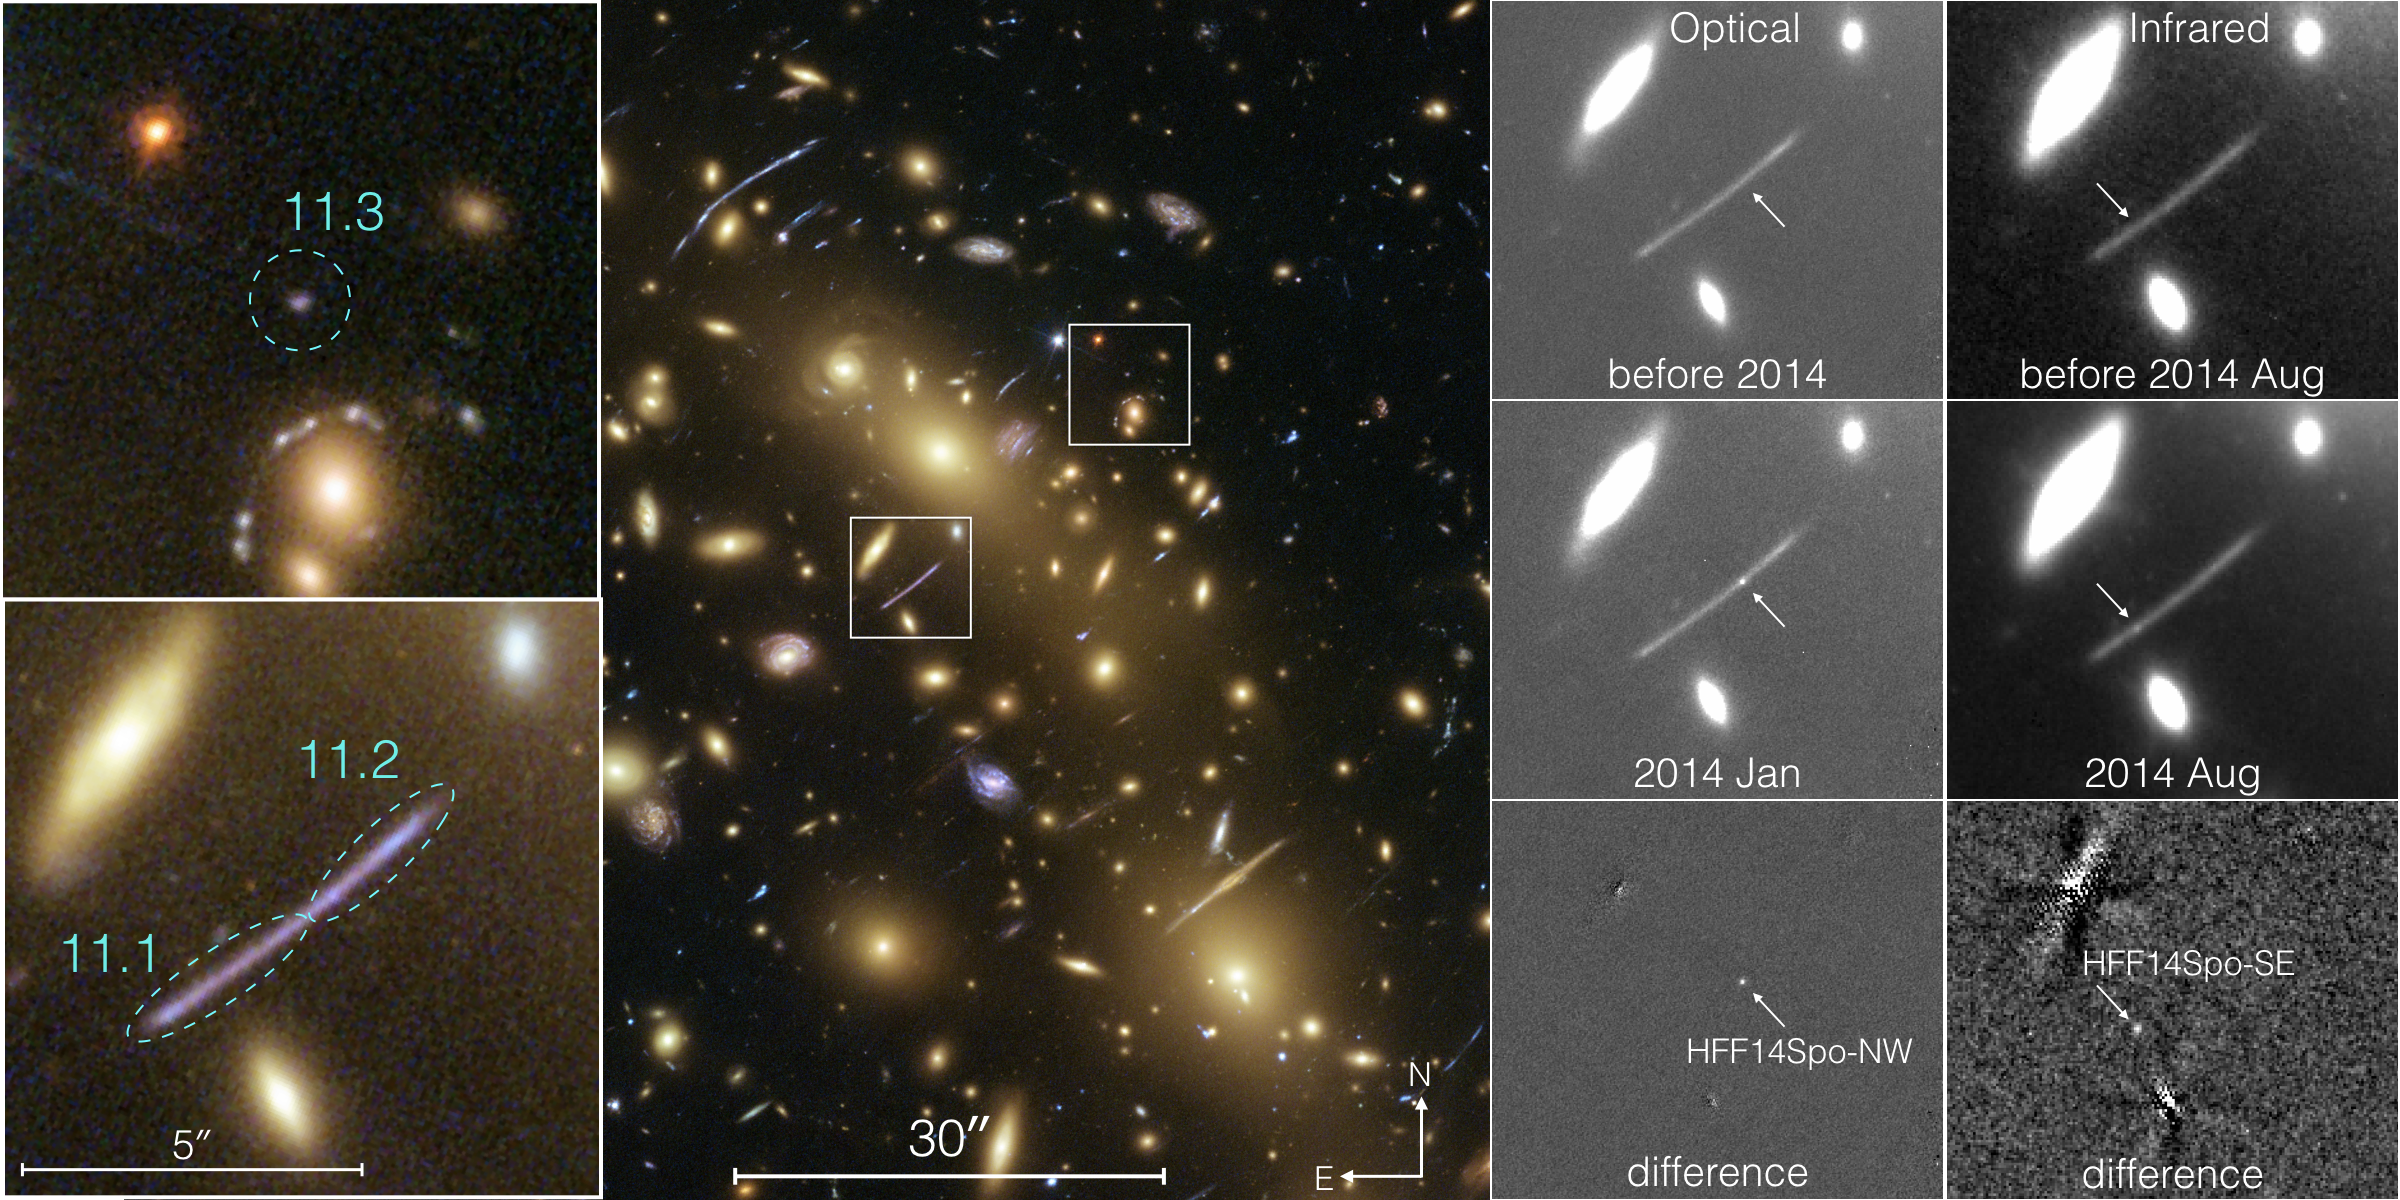
\includegraphics[width=1\textwidth]{./figures/detection_image/detection_image.png}
\caption{ \protect\label{fig:SpockDetectionImages}
The detection of \spockone and \spocktwo in HST imaging from the
Hubble Frontier Fields. The central panel shows the full field of the
MACSJ0416 cluster, in a combined image using optical and infrared
bands from HST.  Two boxes within the main panel demarcate the regions
where the \spock host galaxy images appear. These regions are shown as
two inset panels on the left, highlighting the three images of the
host galaxy (labeled 11.1, 11.2, and 11.3), whcih are caused by the
gravitational lensing of the cluster.  Two columns on the right side
show the discovery of the two transient events in optical and infrared
light, respectively.  In these final two columns the top row is a
template image, the center row shows the epoch when each transient
appeared, and the bottom row is the difference image.
}
\end{center}
\end{figure*}

\begin{figure*}[tbp]
\begin{center}
\includegraphics[width=1\textwidth]{./figures/spock_lightcurves/spock_lightcurves_flux}
\caption{ \protect\label{fig:LightCurves}
Light curves for the two transient events, \spockone\ on the left and \spocktwo\ on the right.  The flux values are rescaled to a zero point of 25 mag. Dates in the observer frame are marked on the top axis, and rest-frame time at z=1.0 is shown on the bottom axis.   As indicated in the legend, optical observations using the \HST\ ACS-WFC detector are plotted as circles in shades of blue and green, while infrared measurements from the WFC3-IR detector are plotted as red, orange and purple squares. 

  }
\end{center}
\end{figure*}

\begin{figure*}[tbp]
  \begin{center}
    \includegraphics[width=\textwidth]{./figures/spock_critical_curves/spock_critical_curves}
    \caption{\protect\label{fig:SpockCriticalCurves}
Locations of the lensing critical curves relative to the positions of
the two \spock sources. Panel (a) marks the \spock locations on the
HST Frontier Fields image of the MACS0416 field in the F814W (I) band.
Panels b-f show magnification maps derived from the Kawamata, Jauzac,
Diego and Zitrin lens models.  All are scaled so that white is $\mu=1$
and black indicates $\mu=1000$.  Panel (g) depicts a trace of the
lensing critical curve near the \spock positions from the GRALE
model. The models shown in b, c and d have separate critical curves
passing near to the two \spock positions. Models in e, f and g have a
single critical curve passing between the two transient locations.
The GLAFIC v3.1 model shown in (c) was defined with the requirement
that multiple critical curves pass through the \spock locations.  All
other panels present the model realization that provides the best fit
to the lensing constraints.
  
}
  \end{center}
\end{figure*}

\begin{figure*}[tbp]
\begin{center}
\includegraphics[width=0.48\textwidth]{./figures/peakluminosity_vs_declinetime/peakluminosity_vs_declinetime_sn}
\includegraphics[width=0.48\textwidth]{./figures/peakluminosity_vs_declinetime/peakluminosity_vs_declinetime_nova_lbv}
\caption{ \protect\label{fig:PeakLuminosityDeclineTime}
Peak luminosity vs. decline time for \spock and other rapidly
declining transients.  Constraints for \spockone and \spocktwo are
plotted as overlapping colored bands, as in
Figure~\ref{fig:PeakLuminosityDeclineTimeWide}.  Two .Ia candidates
are shown as stars \citep{Kasliwal:2010,Poznanski:2010}, and arrows
indicate lower limits for two kilonova
candidates \citep{Perley:2009,Tanvir:2013}.  Grey bands show the MMRD
relation for classical novae, as in
Figure~\ref{fig:PeakLuminosityDeclineTimeWide}.  Circles mark the
observed peak luminosities and decline times for classical novae from
the Milky Way \citep{Downes:2000}, M31 \citep{Shafter:2011}, and the
local group \citep{Kasliwal:2011b}.  Black '+' symbols mark the 7 rapidly declining Recurrent Novae from our own galaxy \citep{Schaefer:2010}, and the large cross labeled at the bottom shows the rapid recurrence nova
M31N 2008-12a \citep{Tang:2014,Darnley:2015}.
}
\end{center}
\end{figure*}

\begin{figure*}[tbp]
  \begin{center}
    \includegraphics[width=\textwidth]{./figures/spock_predictions/spock_predictions}
    \caption{\protect\label{fig:SpockDelayPredictions}
Predictions for the reappearance episodes of both \spockone\ and \spocktwo\, due to gravitational lensing time delays.  The time delays are derived from four independent models of the \macs0416\ cluster, labeled by the modeler's last initial: D=Diego, J=Jauzac, O=Oguri, W=Williams, Z=Zitrin.  The top panel shows photometry collected at the NW position (host galaxy image 11.2) where the first event (\spockone, labeled spock1) appeared in January, 2014.  Optical measurements from ACS are in blue and green, and infrared observations from WFC3-IR are in red and orange, as in Figure~\ref{fig:LightCurves}.  Blue bars in the lower panel show lens models predictions for the dates when that same physical event (\spockone) would have also appeared in the SE location (galaxy image 11.1), due to gravitational lensing time delay.  The lower panel plots photometry from the SE position (11.1). On the right side we see the second observed event (\spocktwo, labeled spock2).  The red bars above show model predictions for when the NW host image 11.2 would have exhibited the gravitationally delayed image of the \spocktwo\ event.
  
  }
  \end{center}
\end{figure*}

%\end{multicols}
\begin{deluxetable}{lccccc}
  \tablewidth{0.7\textwidth}
  \tablecolumns{6}
  \tablecaption{Lens model predictions for time delays and
    magnifications at the observed locations of the \spock
    transients. \label{tab:LensModelPredictions}}
  \tablehead{
    \colhead{Model} &
    \colhead{$\lvert\mu_{\rm NW}\rvert$} & \colhead{$\lvert\mu_{\rm SE}\rvert$} &
    \colhead{$\lvert\mu_{11.3}\rvert$} &  
    \colhead{$\Delta t_{\rm NW:SE}$} & \colhead{$\Delta t_{\rm NW:11.3}$} \\
    \colhead{} & \colhead{} & \colhead{} & \colhead{} & \colhead{(days)} & \colhead{(years)}}
\startdata
CATS &  196$^{+140}_{-53}$ & 46$^{+2}_{-1}$ & 3.3$^{+0.0}_{-0.0}$ & -1.7$^{+2.0}_{-1.9}$ & -3.7$^{+0.1}_{-0.2}$\\[0.5em]
GLAFIC & 29$^{+43}_{-10}$ &  84$^{+103}_{-38}$ &  3.0$^{+0.2}_{-0.2}$ &  4.1$^{+5.5}_{-3.4}$ &  -5.0$^{+0.5}_{-0.6}$\\[0.5em]
GLEE & 182$^{+203}_{-83}$ &  67$^{+31}_{-16}$ &  2.9$^{+0.1}_{-0.1}$ &  36$^{+6}_{-7}$ &  -6.1$^{+0.3}_{-0.2}$\\[0.5em]
GRALE & 13$^{+11}_{-6}$ & 12$^{+9}_{-5}$ & 3.1$^{+2.2}_{-0.9}$ & -10$^{+1}_{-7}$ & -2.5$^{+1.0}_{-3.1}$ \\[0.5em]
SWunited & 38$\pm8$ & 13$\pm1$ & 2.9 $\pm0.1$ & \nodata & \nodata \\[0.5em]
WSLAP$^{+}$ & 35$\pm$20 & 30$\pm$20 & \nodata & -48$\pm$10 & 0.8  \\[0.5em]
ZLTM & 103$^{+48}_{-40}$ & 32$^{+8}_{-10}$ & 3.5$\pm$0.3  & 43$^{+12}_{-10}$ & -3.7$\pm0.3$\\
\enddata
\tablecomments{ Each lens model is identified by the name of the
  modeling team or tool. Time delays give the predicted delay relative
  to an appearance in the NW host image, 11.2. Positive (negative)
  values indicate the NW image is the leading (trailing) image of the
  pair.  The observed time lag between the NW and SE events was
  $\Delta t_{\rm NW:SE}=234\pm6$ days.}
  \label{tab:LensModelPredictions}
\end{deluxetable}

%\begin{multicols}{2}


\begin{methods}
 %Put methods in here.  If you are going to subsection it, use
 %\verb|\subsection| commands.  Methods section should be less than
 %800 words and if it is less than 200 words, it can be incorporated
 %into the main text.
 
 \section{Observations}\label{sec:Observations}

The transient \spock\ was discovered in HST imaging collected as part
of the Hubble Frontier Fields (HFF) survey (HST-PID:13496, PI:Lotz), a
multi-cycle program observing 6 massive galaxy clusters and associated
``blank sky'' parallel fields.  Several HST observing programs have
provided additional observations supplementing the core HFF program.
One of these is the FrontierSN program (HST-PID:13386, PI:Rodney),
which aims to identify and study explosive transients found in the HFF
and related programs.  The FrontierSN team discovered \spock\ in two
separate HFF observing campaigns on the galaxy cluster
\MACS0416\ (hereafter, MACS0416).  The first was an imaging campaign
in January, 2014 during which the MACS0416 cluster field was observed
in optical bands using the Advanced Camera for Surveys Wide Field
Camera (ACS-WFC).  The second concluded in August, 2014, and imaged
the cluster with the infrared detector of HST's Wide Field Camera 3
(WFC3-IR).

To discover transient sources, the FrontierSN team processes each new
epoch of HST data through a difference imaging
pipeline\footnote{\url{https://github.com/srodney/sndrizpipe}}, using
archival HST images to provide reference images (templates) which are
subtracted from the astrometrically registered HFF images. In the case
of MACS0416, the templates were constructed from images collected as
part of the Cluster Lensing And Supernova survey with Hubble (CLASH,
HST-PID:12459, PI:Postman). The resulting difference images are
visually inspected for new point sources, and any new transients of
interest (primarily supernovae, SNe) are followed up with additional
HST imaging or ground-based spectroscopic observations as needed.  For
a more complete description of the operations of the FrontierSN
program, see \citet{Rodney:2015b}.

The follow-up observations for \spock\ included HST observations in
infrared and optical bands using the WFC3-IR and ACS-WFC detectors,
respectively, as well as spectroscopy of the \spock\ host galaxy using
the Very Large Telescope (VLT) and the Visible Multi-object
Spectrograph (VIMOS, \textcolor{red}{citation?}), and also using the
X-Shooter cross-dispersed echelle spectrograph
\citep{Vernet:2011}. The X-Shooter observations
(\textcolor{red}{Program ID?}, PI:Hjorth) were taken on October 19th,
21st and 23rd (2014) for a total of 4.5 hours, with the slit centered
on the position of \spock2.  The spectrum did not provide any
detection of the transient source itself (as we will see below, it had
already faded back to its quiescent state by that time).  However, it
did provide an unambiguous redshift for the host galaxy of
$z=1.0054\pm0.0002$ from \Ha\ and \ion{O}{[ii]}.  These line
identifications are consistent with two measures of the photometric
redshift of the host: $z=1.00+-0.02$ from the BPZ algorithm
\citep{Benitez:2000}, and $z=0.92\pm0.05$, derived using the EAZY
program \citep{Brammer:2008}.


TODO: add a table with photometry.


  
  

  
  
 \subsection{Gravitational Lens Models}\label{sec:LensingModels}


%That same transient episode would have appeared at
%different times in host galaxy images 11.1 and 11.3, due primarily to
%the \citet{Shapiro:1964} delay.  The $\Delta t_{\rm NW:SE}$ column in
%Table~\ref{tab:LensModelPredictions} gives the model predictions for
%the number of days between the appearance of the \spockone\ event in
%the NW host image (11.2) and the date when it should have been
%observable in the adjacent SE host image (11.1).  The opposite value
%would give the time difference between the August 2014
%\spocktwo\ event and its expected appearance in host image 11.2.
%Table~\ref{tab:LensModelPredictions} also reports the predicted time
%delay (in years) between appearance in the NW host image 11.2 and the
%more widely separated image 11.3.

The six lens models used to provide estimates of the plausible range
of magnifications and time delays are:

\bigskip
\begin{itemize}
\item{{\it CATS:} The model of \citet{Jauzac:2014}, generated with
  the {\tt LENSTOOL} software
  \citep{Jullo:2007},\footnote{\url{http://projects.lam.fr/repos/lenstool/wiki}}}
  using strong lensing constraints.  This model makes a
  light-traces-mass assumption and parameterizes cluster and galaxy components
  using psuedo-isothermal elliptical mass distribution (PIEMD) density profiles
  \citep{Eliasdottir:2007}.
\item{\it GLAFIC:} The model of \citet{Kawamata:2016}, built using
  the {\tt
    GLAFIC}\footnote{\url{http://www.slac.stanford.edu/~oguri/glafic/}}
  software \citep{Oguri:2010b} with strong-lensing constraints. This
  model assumes simply parametrized mass distributions, and model
  parameters are constrained using positions of more than 100 multiple
  images.
\item{{\it GRALE:} A free-form, adaptive grid model developed using
  the GRALE software tool \citep{Liesenborgs:2006, Liesenborgs:2007,
    Mohammed:2014, Sebesta:2016}, which implements a genetic algorithm
  to reconstruct the cluster mass distribution with projected Plummer
  \citeyear{Plummer:1911} density profiles.}
\item{\it SWUnited:} The model of \citet{Hoag:2016}, built using the
  {\tt SWUnited} modeling method \citep{Bradac:2005, Bradac:2009}, in
  which an adaptive pixelated grid iteratively adapts the mass
  distribution to match both strong- and weak-lensing constraints.
  Time delay predictions are not available for this model.
\item{\it WSLAP+:} Created with the {\tt WSLAP+} software
  \citep{Sendra:2014}: Weak and Strong Lensing Analysis Package plus
  member galaxies (Note: no weak-lensing constraints used for this
  MACS J0416 model). Interactive online model exploration available at
  \url{http://www.ifca.unican.es/users/jdiego/LensExplorer}.
\item{{\it Z-LTM:} A model with strong- and weak-lensing constraints,
  built using the ``light-traces-mass'' (LTM) methodology
  \citep{Zitrin:2009a,Zitrin:2015}, first presented for MACS0416 in
  \citet{Zitrin:2013a}.}
\end{itemize}
\bigskip    

Early versions of the {\it SWUnited}, {\it CATS}, {\it Z-LTM} and {\it
  GRALE} models were originally distributed as part of the Hubble
Frontier Fields lens modeling project,\footnote{For more details, see
  \url{https://archive.stsci.edu/prepds/frontier/lensmodels/}} in
which models were generated based on data available before the start
of the HFF observations to enable rapid early investigations of lensed
sources. The versions of these models applied here are updated to
incorporate additional lensing constraints.  In all cases the lens
modelers made use of strong-lensing constraints (multiply-imaged
systems and arcs) derived from HST imaging collected as part of the
CLASH program (PI:Postman, HST PID:12459,
\citealt{Postman:2012}). These models also made use of spectroscopic
redshifts in the cluster field from \citet{Mann:2012},
\citet{Christensen:2012}, and \citet{Grillo:2015a}.  The {\it Diego}
and {\it Kawamata} models presented here made use of the catalog of
spectroscopic redshifts and multiply-imaged background galaxies from
\citep{Caminha:2016}.  Input weak-lensing constraints were derived
from data collected at the Subaru Telescope by PI K. Umetsu (in prep)
and archival imaging.
%\citet{Priewe:2016} provides a more complete
%description of the methodology of model and a comparison of the
%magnification predictions and uncertainties across the entire
%\macs0416 field.

The locations of critical curves for for a source at $z=1$ (the
redshift of the \spock host galaxy) are shown in
Figure~\ref{fig:SpockCriticalCurves}. In some cases the best-fit model
predicts that a single critical curve passes between the two \spock
locations, as would be expected if the host arc is indeed composed of
two elongated images of the host galaxy. Other models can accommodate
a lensing scenario that brings multiple critical curves across the two
spock locations. 

Figure~\ref{fig:LensModelContours} presents probability distributions
derived from these models for the three magnifications and two time
delay values of interest.  These distributions were derived by
combining the Monte Carlo chains from the CATS, GLAFIC, GRALE and
Z-LTM models, with weighting applied to account for the different
number of model iterations in each chain. Four of the five models
agree that host image 11.3 is the leading image, appearing some 2--6
years before the other two images.  The models do not agree on the
arrival sequence of images 11.1 and 11.2: some have the NW image 11.2
as a leading image, and others have it as a trailing image.  However,
the models do consistently predict that the separation in time between
those two images should be roughly in the range of 1 to 60 days.


%The angular separation of $1\farcs8$ between the \spock events
%corresponds to a physical separation of many tens of parsecs in the
%source plane.  A star could not traverse that distance in the
%$\sim$120 rest-frame days that separate the two \spock events.  Thus,
%even with a critical curve smeared out by the effects of the ICL, it
%would be impossible for a single star crossing a single caustic in the
%source plane to be responsible for both transients.

 \subsection{X-ray Non-detections}\label{sec:Xray}

The \MACS0416 field was observed by the SWIFT X-Ray Telescope (XRT) and
UltraViolet/Optical Telescope (UVOT) in April 2013.  No source was
detected near the locations of the \spock events (N. Gehrels, private
communication).  The field was also observed by the Chandra X-ray
space telescope with the ACIS-I instrument for three separate
programs.  On June 7, 2009 it was observed for GO program 10800770
(PI: H.\,Ebeling).  It was revisited for GTO program 15800052 (PI:
S.\,Murray) on November 20, 2013 and for GO program 15800858 (PI: C.\,
Jones) on June 9, August 31, November 26, and December 17, 2014. These
Chandra images show no evidence for an x-ray emitting point source
near the \spock locations on those dates (S. Murray, private
communication). 

 \subsection{Light Curve Fitting}\label{sec:LightCurves}

Due to the rapid decline timescale, no observations were collected for
either event that unambiguously show the declining portion of the
light curve. Therefore, we must make some assumptions for the shape of
the light curve in order to quantify the peak luminosity and the
corresponding timescales for the rise and the decline.  We first
approach this with a simplistic model that is piece-wise linear in
magnitude vs time.  Figure~\ref{fig:LinearLightCurveFits} shows
examples of the resulting fits for the two events.  For each fit we
use only the data collected within 3 days of the brightest observed
magnitude, which allows us to fit a linear rise separately for the
F606W and F814W light curves for \spockone and the F125W and F160W
light curves for \spocktwo. To quantify the covariance between the
true peak brightness, the rise time and the decline timescale, we use
the following procedure:

\begin{enumerate}
\item make an assumption for the date of peak, $t_{\rm pk}$;
\item measure the peak magnitude at $t_{\rm pk}$ from the linear fit
  to the rising light curve data;
\item assume the source reaches a minimum brightness (maximum
  magnitude) of 30 AB mag at the epoch of first observation after the
  peak;
\item draw a line for the declining light curve between the assumed
  peak and the assumed minimum brightness;
\item use that declining light curve line to measure the timescale for
  the event to drop by 2 magnitudes, $t_2$;
\item make a new assumption for $t_{\rm pk}$ and repeat.
\end{enumerate}

As shown in Figure~\ref{fig:LinearLightCurveFits}, the resulting
piece-wise linear fits are simplistic, but nevertheless approximately
capture the observed behavior for both events.  Furthermore, since
this toy model is not physically motivated, it allows us to remain
agnostic for the time being as to the astrophysical source(s) driving
these transients.  From these fits we can see that \spockone most
likely reached a peak magnitude between 25 and 26.5 AB mag in both
F814W and F435W, and had a decline timescale $t_2$ of less than 2 days
in the rest-frame. The observations of \spocktwo provide less
stringent constraints, but we see that it had a peak magnitude between
23 and 26.5 AB mag in F160W and exhibited a decline time of less than
seven days.  These fits also illustrate the generic fact that a higher
peak brightness corresponds to a longer rise time and a faster decline
timescale, independent of the specific model used.  Changes to the
arbitrary constraints we placed on these linear fits do not
substantially affect these results.

At any assumed value for the time of peak brightness this linear
interpolation gives an estimate of the peak magnitude. We then convert
that to a luminosity (e.g., $\nu L_\nu$ in erg s$^{-1}$) by first
correcting for the luminosity distance assuming a standard \LCDM
cosmology, and then accounting for an assumed lensing magnification,
$\mu$.  The range of plausible lensing magnifications ($10<\mu<100$)
is derived from the union of our six independent lens models (Methods,
Figure~\ref{fig:LensModelContours}).  This results in a grid of
possible peak luminosities for each event as a function of
magnification and time of peak.  As we are using linear light curve
fits, the assumed time of peak is equivalent to an assumption for the
decline time, which we quantify as $t_2$, the time over which the
transient declines by 2 magnitudes.




 \subsection{Host Galaxy}\label{sec:HostGalaxy}

To examine whether the two transients originated from the same
physical location in the source plane, we looked for differences in
the properties of the \spock host galaxy at the location of each
event.  We first used the technique of ``pixel-by-pixel'' SED fitting
as described in \citet{Hemmati:2014} to determine rest-frame colors
and stellar properties in a single resolution element of the \HST
imaging data.  For this purpose we used the deepest possible stacks of
\HST images, comprising all available data except those images where
the transient events were present.  The resulting maps of stellar
population properties are shown in Figure~\ref{fig:HostProperties}.
Table~\ref{tab:HostProperties} reports measurements of the three
derived stellar population properties (color, mass, age) from host
images 11.1, 11.2 and 11.3.  In 11.1 and 11.2 these measurements were
extracted from the central pixel at the location of each of the two
\spock events.  The lensing magnification here ranges from
$\mu=10$ to 100 (see Section~\ref{sec:LensingModels}), corresponding
to a size on the source plane between 6 and 600 pc$^2$.  For host
image 11.3 we report the stellar population properties derived from
the pixel at the center of the galaxy, because the lens models do not
have sufficient precision to map the \spock locations to specific
positions in image 11.3.  With a magnification of $\sim$3 to 5, this
extraction region covers roughly 2000 to 6000 pc$^2$.

\begin{deluxetable}{lccc}
  \tablewidth{\linewidth}
  \tablecolumns{6}
  \tablecaption{Properties of the local stellar population in the \spock host galaxy, from SED fitting.}
  \tablehead{ {Host image:} & \colhead{11.1} & \colhead{11.2} & \colhead{11.3}\\
{Location:}   & \colhead{\spocktwo} & \colhead{\spockone} & \colhead{center}}
\startdata
$(U-V)_{\rm rest}$            & 0.69$^{+0.2}_{-0.05}$  & 0.52$^{+0.15}_{-0.10}$      & 0.39$\pm$0.05  \\
$\log[\Sigma (M_*/\Msun)]$  & 7.14 $\pm$ 0.15   & 7.14 $\pm$ 0.15     & 7.04 $\pm$ 0.10   \\
Age (Gyr)                   & 0.292$\pm$0.5 &   0.290$\pm$0.5 &  0.292$\pm$0.5  
\enddata
\label{tab:HostProperties}
\end{deluxetable}

The reported uncertainties for these derived stellar properties in
Table~\ref{tab:HostProperties} reflect only the measurement errors
from the SED fitting, and do not attempt to quantify potential
systematic biases.  Such biases could arise, for example, from color
differences in the background light, which is dominated by the cluster
galaxies and varies significantly across the \MACS0416 field.  Such a
bias might shift the absolute values of the parameter scales for any
given host image (e.g., making the galaxy as a whole appear bluer,
more massive and younger). However, the gradients across any single
host image are unlikely to be driven primarily by such systematics.

Figure~\ref{fig:HostProperties} and Table~\ref{tab:HostProperties}
show that the measured values of the color, stellar mass, and age at
the two \spock locations are mutually consistent. Thus, it is
plausible to assume that the two positions map back to the same
physical location at the source plane.  Comparing those two locations
to the center of the galaxy as defined in image 11.3, we see only a
mild tension in the rest-frame U-V color. This comparison therefore
cannot quantitatively rule out the possibility that the two transient
events are located at the center of the galaxy. However, the maps
shown in Figure~\ref{fig:HostProperties} do show a gradient in both
U-V color and stellar age. For both images 11.1 and 11.2 the bluest
and youngest stars (U-V$\sim$0.3, $\tau\sim$280 Myr) are localized in
knots near the extreme ends of each image, well separated from either
of the \spock transient events.  In the less distorted host image 11.3
the bluer and younger stars are concentrated near the center. Taken
together, these color and age gradients suggest that the two
transients are not coincident with the center of their host galaxy.

\begin{deluxetable*}{rllc ccc ccc c}
  \tablewidth{\linewidth}
  \tablecolumns{12}
  \tablecaption{Measurements of the \ionline{O}{[ii]} $\lambda\lambda$3626,3629 lines from \spock host galaxy images 11.1 and 11.2\tablenotemark{a}}
  \tablehead{ \colhead{Aperture} & \colhead{R.A.} & \colhead{Dec.} & \colhead{distance to} &  \multicolumn{3}{c}{\ionline{O}{[ii]} $\lambda$3726} & \multicolumn{3}{c}{\ionline{O}{[ii]} $\lambda$3729} & \colhead{Line}\\
    \colhead{ID} & \colhead{J2000} & \colhead{J2000} & \colhead{\spocktwo} & \colhead{Flux} & \colhead{$\lambda_{\rm center}$} & \colhead{FWHM} &
    \colhead{Flux} & \colhead{$\lambda_{\rm center}$} & \colhead{FWHM} & \colhead{Ratio}\\
    & \colhead{(degrees)} & \colhead{(degrees)} & \colhead{(Arcsec)} & \colhead{(erg\,s$^{-1}$\,cm$^{-2}$)} & \colhead{(\AA)} & \colhead{(\AA)} &
    \colhead{(erg\,s$^{-1}$\,cm$^{-2}$)} & \colhead{(\AA)} & \colhead{(\AA)}}
\startdata
    1  & 64.039371 &  -24.070450 &  -1.54 & 2.19e-18 &   7472.37 &  4.00 &    3.57e-18 &   7478.17 & 4.00 &      1.63\\      
    2  & 64.039218 &  -24.070345 &  -0.88 & 4.73e-18 &   7472.16 &  4.00 &    5.30e-18 &   7478.12 & 3.40 &      1.12\\
    3  & 64.039078 &  -24.070264 &  -0.30 & 5.05e-18 &   7472.29 &  4.00 &    6.10e-18 &   7478.27 & 3.73 &      1.21\\
    4  & 64.038921 &  -24.070163 &   0.39 & 4.22e-18 &   7472.19 &  4.00 &    5.74e-18 &   7478.08 & 3.59 &      1.36\\
    5  & 64.038785 &  -24.070078 &   0.97 & 3.86e-18 &   7472.25 &  4.00 &    6.56e-18 &   7478.19 & 4.00 &      1.70\\
    6  & 64.038637 &  -24.069958 &   1.65 & 4.80e-18 &   7472.51 &  4.00 &    5.42e-18 &   7478.07 & 2.69 &      1.13\\
    7  & 64.038501 &  -24.069865 &   2.24 & 4.60e-18 &   7472.57 &  3.43 &    5.74e-18 &   7478.17 & 3.20 &      1.25\\
    8  & 64.038352 &  -24.069752 &   2.92 & 4.70e-18 &   7472.54 &  3.54 &    6.22e-18 &   7478.16 & 2.95 &      1.32\\
    9  & 64.038229 &  -24.069648 &   3.50 & 3.26e-18 &   7472.83 &  2.80 &    5.79e-18 &   7478.16 & 2.84 &      1.77\\
   10  & 64.038076 &  -24.069532 &   4.19 & 2.44e-18 &   7473.01 &  2.57 &    3.22e-18 &   7478.10 & 2.73 &      1.32\\
Spo-1  & 64.038565 &  -24.069939 &   1.90 & 4.30e-18 &   7472.55 &  3.13 &    5.49e-18 &   7478.01 & 2.89 &      1.28\\
Spo-2  & 64.038998 &  -24.070241 &   0.00 & 4.37e-18 &   7472.46 &  4.00 &    6.10e-18 &   7478.22 & 3.79 &      1.40\\
\enddata

\tablenote{Properties of the of the \ionline{O}{[ii]} lines were
  derived from 1-D spectra extracted from the MUSE data cube at 10
  locations spaced 0\farcs6 apart along the length of the arc that
  comprises images 11.1 and 11.2 of the \spock host galaxy. Each
  extraction used an aperture of 0\farcs6 radius, centered on the
  mid-line of the host galaxy arc. The integrated line flux, observed
  wavelength of line center ($\lambda_{\rm center}$), and full width
  at half maximum (FWHM) were found by fitting a Gaussian profile to
  each component of the doublet.}
\label{tab:MuseLineFits}
\end{deluxetable*}


%#   ID   RA        DEC       Delta_spock2  OII]3726                                                                   OII]3729                                                                 OII]3729/OII]3726
%#                              Arcsec      Flux(erg/s/cm^2)  Center(Angstrom) Amplitude(erg/s/cm^2) FWHM(Angstrom)    Flux(erg/s/cm^2)  Center(Angstrom) Amplitude(erg/s/cm^2) FWHM(Angstrom)   
%#  ID    RA         DEC        d_spock2  flux3726           wave3726           amplitude3726       fwhm3726         flux3729           wave37269           amplitude3729       fwhm3729        fluxratio3729to3726


In addition to the \HST imaging data, we also have spatially resolved
spectroscopy from the MUSE integral field data. The only significant
spectral line feature for the \spock host is the \forbidden{O}{ii}
($\lambda\lambda$ 3727, 3729) doublet, observed at 7474 and 7478
\AA. Figure~\ref{fig:MUSEOIISequence} shows the observed
\forbidden{O}{ii} lines at 10 positions along the length of the arc,
which comprises images 11.1 and 11.2. Each extraction has been
normalized to show a peak line flux at unity, so that the line
profiles and the doublet line ratios may be more easily compared.  At
each position the lines were extracted using apertures with a radius
of 0\farcs6, so adjacent extractions are not independent, although the
two extractions centered on the \spockone and -SE positions have no
overlap.

From each extracted 1-D spectrum the integrated line flux, observed
wavelength of line center ($\lambda_{\rm center}$), and full width at
half maximum (FWHM) were found by fitting a Gaussian profile to each
component of the doublet.  Properties derived from these line fits are
reported in Table~\ref{tab:MuseLineFits}. The \forbidden{O}{ii} lines
do not exhibit any discernible gradient across the host galaxy images
in terms of the wavelength of line centers, full width at half
maximum, or the intensity ratio of the two components of the doublet.
Thus, the \forbidden{O}{ii} measurements from MUSE cannot be used to
distinguish either \spock location from the other, or to definitively
answer whether either position is coincident with the center of the
host galaxy.  We conclude that it is plausible but not certain that
the two \spock events arose from the same physical location in the
host galaxy.




 \subsection{Luminous Blue Variable Light Curve Comparison}
\label{sec:LBVlightcurves}

Extended Data Fig.~\ref{fig:LBVLightCurveComparison} presents a direct
comparison of the observed \spock light curves against the light
curves of the two LBVs that have well-studied rapid eruptions: SN
2009ip and NGC3432-LBV1. The brief outbursts of these LBVs have been
less finely sampled than the two \spock events, but the available data
show a wide variety of rise and decline times, even for a single
object over a relatively narrow time window of a few months.


\subsection{LBV Build-up timescale}\label{sec:LBVbuildup}

To explore some of the physical implications of an LBV classification
for the two \spock events, we first make a rough estimate of the total
radiated energy, which can be computed using the decline timescale
$t_2$ and the peak luminosity $L_{\rm pk}$:

\begin{equation}
  \label{eqn:Erad}
  E_{\rm rad} = \zeta \t2 \Lpk,
\end{equation}

\noindent where $\zeta$ is a dimensionless factor of order unity that
depends on the precise shape of the light curve\cite{Smith:2011b}. Note that
 earlier work\cite{Smith:2011b} has used $t_{1.5}$ instead of $t_2$, which amounts to
  a different light curve shape term, $\zeta$.  Adopting
\Lpk$\sim10^{41}$ erg s$^{-1}$ and \t2$\sim$1 day (as shown in
Figure~\ref{fig:PeakLuminosityDeclineTime}), we find that the total
radiated energy is $E_{\rm rad}\sim10^{46}$ erg.  A realistic range
for this estimate would span $10^{44}<E_{\rm rad}<10^{47}$ erg, due to
uncertainties in the magnification, bolometric luminosity correction,
decline time, and light curve shape. These uncertainties
notwithstanding, our estimate falls well within the range of
plausible values for the total radiated energy of a major LBV
outburst.

The ``build-up'' timescale\citep{Smith:2011b} matches the radiative
energy released in an LBV eruption event with the radiative energy
produced during the intervening quiescent phase:

\begin{equation}
  \label{eqn:trad}
t_{\rm rad} = \frac{E_{\rm rad}}{L_{\rm qui}} = \t2 \frac{\xi\Lpk}{L_{\rm qui}},
\end{equation}

\noindent where $L_{\rm qui}$ is the luminosity of the LBV progenitor
star during quiescence.

The \spock events are not resolved as individual stars in their
quiescent phase, so we have no useful constraint on the quiescent
luminosity. Thus, instead of using a measured quiescent luminosity to
estimate the build-up timescale, we assume that $t_{\rm rad}$ for
\spock corresponds to the observed rest-frame lag between the two
events, roughly 120 days (this accounts for both cosmic time dilation
and a gravitational lensing time delay of $\sim$40 days). Adopting
$\Lpk=10^{41}$ erg s$^{-1}$ and $\t2=2$ days (see
Figure~\ref{fig:PeakLuminosityDeclineTime}), we infer that the
quiescent luminosity of the \spock progenitor would be $L_{\rm
  qui}\sim10^{39.5}$ erg s$^{-1}$ ($M_V\sim-10$).


%Rapid transient episodes in LBVs may
%best be explained by a sudden ejection of an optically thick shell
%\citep[e.g.,][]{Smith:2010, Smith:2011b}, or by some form of S
%Dor-type variability \citep{Weis:2005, VanDyk:2006, Foley:2011}, which
%may be driven by stellar pulsation rather than mass ejection
%\citep{VanGenderen:1997, VanGenderen:2001}.  For massive stars such as
%\etacar at its great eruption and the rapidly varying SN 2009ip, the
%effective photospheric radius during eruption must have been
%comparable to the orbit of Saturn \citep[$10^{14}$
%  cm;][]{Davidson:1997, Smith:2011b, Foley:2011}.  With observed
%photospheric velocities of order 500 km s$^{-1}$ for such events, the
%dynamical timescale of the extended photosphere is on the order of
%tens to hundreds of days.  The very rapid light curves of both \spock
%events would push down the lower limit of this range to just a few
%days.  If these are indeed LBV eruptions, then they are near the
%extreme limit of what is physically possible for such massive stellar
%eruptions.




%To examine the temperature and total energy output, we first make a
%set of (admittedly unfounded) assumptions: (1) the two outbursts had a
%very similar SED; (2) the last observed epoch for each event
%corresponds to the same phase relative to the true epoch of peak
%brightness; and (3) the lensing magnifications for the two events are
%the same.  These simplifying assumptions allow us to jointly apply the
%optical observations of \spockone and the NIR observations of
%\spocktwo as constraints on the SED in any given epoch.  We then set
%an assumption for the epoch of peak brightness, make another
%assumption for the magnification of both events, and then fit a
%blackbody to the resulting extrapolated SED. From this blackbody fit
%we derive a temperature and integrate to get an estimate of the
%pseudo-bolometric luminosity.  The resulting inferred physical
%parameters are plotted in Figure~\ref{fig:DerivedPhysicalParameters}.


 \subsection{RN Light Curve Comparison}\label{sec:RNLightCurves}

%Nova outbursts can exhibit decline times from
%$\sim$1 day to many months, so the timescale of the \spock light
%curves can easily be accommodated by the nova scenario.
%However, the rise time of the \spock events is somewhat out of the ordinary for
%nova outbursts.  In particular, for recurrent nova eruptions that
%decline rapidly ($t_2<10$ days) they tend to also reach peak
%brightness very quickly, on timescales $<1$ day
%\citep{Schaefer:2010}. The 2014 eruption of the rapid-recurrence nova
%M31N 2008a-12 reached maximum brightness in a little under 1 day
%\citep{Darnley:2015}.  However, the rise time for nova eruptions is
%poorly constrained, as rapid-cadence imaging is rarely secured until
%after an initial detection near peak brightness.  Unlike the situation
%with a kilonova light curve, there is no a priori physical expectation
%for an especially rapid rise to peak in nova light curves.

There are ten known RNe in the Milky Way galaxy, and seven of
these exhibit outbursts that decline rapidly, fading by two magnitudes
in less than ten days \citep{Schaefer:2010}. 
% U Sco, V2487 Oph, V394 CrA, T CrB, RS Oph, V745  Sco, and V3890 Sgr.
Figure~\ref{fig:RecurrentNovaLightCurveComparison} compares the \spock
light curves to a composite light curve (the gray shaded region),
which encompasses the V band light curve templates
\citep{Schaefer:2010} for all seven of these galactic RN events.  The
Andromeda galaxy (M31) also hosts at least one RN with a rapidly
declining light curve.  The 2014 eruption of this well-studied nova,
M31N 2008-12a, is shown as a solid black line in
Figure~\ref{fig:RecurrentNovaLightCurveComparison}, fading by 2 mags
in less than 3 days.  This comparison demonstrates that the rapid
decline of both of the \spock transient events is fully consistent
with the eruptions of known RNe in the local universe.

%Among the most luminous classical novae known, a similarly rapid
%decline time is not unheard of.  For example, the bright nova
%M31N-2007-11d had $t_2 = 9.5$ days \citep{Shafter:2009}.  The
%extremely luminous nova SN 2010U had $t_2 = 3.5 \pm 0.3$
%\citep{Czekala:2013}.  The nova L91 required at least 4 days to rise
%to maximum \citep{Shafter:2009}, and then declined with $t_2 = 6 \pm
%1$ days \citep{DellaValle:1991, Williams:1994, Schwarz:2001}.


\subsection{RN Luminosity and Recurrence Period}\label{sec:RNLuminosityRecurrence}

To examine the recurrence period and peak brightness of the \spock
events relative to RNe, we rely on a pair of papers that evaluated an
extensive grid of nova models through multiple cycles of outburst and
quiescence \citep{Prialnik:1995,Yaron:2005}.
Figure~\ref{fig:RecurrentNovaRecurrenceComparison} plots first the RN
outburst amplitude (the apparent magnitude between outbursts minus the
apparent magnitude at peak) and then the peak luminosity against the
log of the recurrence period in years.
% The observations for \spock 
% are shown in comparison to observed RNe (crosses) and theoretical
% models (circles) from \citet{Yaron:2005}.
For the \spock events we can only measure a lower limit on the
outburst amplitude, since the presumed progenitor star is unresolved,
so no measurement is available at
quiescence. Figure~\ref{fig:RecurrentNovaRecurrenceComparison} shows
that a recurrence period as fast as one year is expected only for a RN
system in which the primary white dwarf is both very close to the Chandrasekhar
mass limit (1.4 \Msun) and also has an extraordinarily rapid mass
transfer rate ($\sim10^{-6}$ \Msun yr$^{-1}$).  The models of
\citet{Yaron:2005} suggest that such systems should have a very low
peak amplitude (barely consistent with the lower limit for \spock) and
a low peak luminosity ($\sim$100 times less luminous than the \spock
events).

The closest analog for the \spock events from the population of known
RN systems is the nova M31N\,2008-12a.  \citet{Kato:2015} provided a
theoretical model that can account for the key observational
characteristics of this remarkable nova: the very rapid recurrence
timescale ($<$1 yr), fast optical light curve ($\t2\sim2$ days), and
short supersoft x-ray phase \citep[6-18 days after optical
  outburst][]{Henze:2015a}.  To match these observations,
\citeauthor{Kato:2015} invoke a 1.38 \Msun white dwarf primary,
drawing mass from a companion at a rate of $1.6\times10^{-7}$ \Msun
yr$^{-1}$.  This is largely consistent with the theoretical
expectations derived by \citet{Yaron:2005}, and reinforces the
conclusion that a combination of a high mass white dwarf and efficient
mass transfer are the key ingredients for rapid recurrence and short
light curves. The one feature that cannot be effectively explained
with this hypothesis is the peculiarly high luminosity of the \spock
events -- even after accounting for the very large uncertainties. 

 \input{Microlensing}
 \subsection{Color Curves}\label{sec:ColorCurves}

At redshift $z=1$ the observed optical and infrared bands translate to
rest-frame ultraviolet (UV) and optical wavelengths, respectively.  To
derive rest-frame UV and optical colors from the observed photometry,
we start with the measured magnitude in a relatively blue band (F435W
and F606W for \spockone and F105W, F125W, F140W for \spocktwo).  We
then subtract the coeval magnitude for a matched red band (F814W for
\spockone, F125W or F160W for \spocktwo), derived from the linear fits
to those bands.  To adjust these to rest-frame filters, we apply K
corrections\citep{Hogg:2002}, which we compute by
defining a crude SED via linear interpolation between the observed
broad bands for each transient event at each epoch.  For consistency
with past published results, we include in each K correction a
transformation from AB to Vega-based magnitudes.  The resulting UV and
optical colors are plotted in Figure~\ref{fig:ColorCurves}.  Both
\spockone and \spocktwo show little or no color variation over the
period where color information is available.  This lack of color
evolution is compatible with all three of the primary hypotheses
advanced, as it is possible to have no discernible color evolution
from either an LBV or RN over this short time span, and microlensing
events inherently exhibit an unchanging color.

If these two events are from a single source then one could construct
a composite SED from rest-frame UV to optical wavelengths by combining
the NW and SE flux measurements, but only after correcting for the
relative magnification.  Figure~\ref{fig:LightCurves} shows that the
observed peak brightnesses for the two events agree to within
$\sim30\%$.  This implies that for any composite SED, the rest-frame
UV to optical flux ratio is approximately equal to the NW:SE
magnification ratio, and any extreme asymmetry in the magnification
would indicate a very steep slope in the SED.

 \subsection{Rates}\label{sec:RatesMethods}

To derive a rough estimate of the rate of \spock-like transients, we
first define the set of strongly lensed galaxies in which a similarly
faint and fast transient could have been detected in the HFF
imaging. The single-epoch detection limit of the HFF transient search
was $m_{\rm lim}=26.7$ AB mag, consistent with the SN searches carried
out in the CLASH and CANDELS programs\cite{Graur:2014,Rodney:2014}.
For a transient with peak brightness $M_{V}>-14$ mag to be detected,
the host galaxy must be amplified by strong lensing with a
magnification $\mu>20$ at $z\sim1$, growing to $\mu>100$ at $z\sim2$.
Using photometric redshifts and magnifications derived from the GLAFIC
lens models the six HFF clusters, we find $N_{\rm gal}=6$ galaxies
that satisfy this criterion, with redshifts $0.5<z<1.5$ (Extended Data
Fig.~\ref{fig:StronglyLensedGalaxies}).

We then define the {\it control time}, $t_{c}$, for the HFF survey,
which gives the span of time over which each cluster was observed with
a cadence sufficient for detection of such rapid transients.  We
define this as any period in which at least two \HST observations were
collected within every ten day span. This effectively includes the
entirety of the primary HFF campaigns on each cluster, but excludes
all of the ancillary data collection periods from supplemental \HST
imaging programs. The average control time for an HFF cluster is
$t_{c}$=0.22 years (80 days).  Treating each \spock event as a
separate detection, we can derive a rate estimate using $R = 2 /
(N_{\rm gal}\,t_c)$.  This yields $R=1.5$ events galaxy$^{-1}$
year$^{-1}$.   

Future examination of the rate of such transients should consider the
total stellar mass and the star formation rates of the galaxies
surveyed, or use a projection of the lensed background area onto the
source plane to derive a volumetric rate.  Such analyses would require
a more detailed exploration of the impact of lensing uncertainties on
derived properties of the lensed galaxies and the lensed volume, and
this is beyond the scope of current work.


 
\end{methods}

% Supplemental figures
\input{Supplemental}


%% Put the bibliography here, most people will use BiBTeX in
%% which case the environment below should be replaced with
%% the \bibliography{} command.

\bibliography{./bibliography/biblio}{}



%% Here is the endmatter stuff: Supplementary Info, etc.
%% Use \item's to separate, default label is "Acknowledgements"

\begin{addendum}
 %\item[Supplementary Information] 
 \item 
\begin{acknowledgments}
The authors thank Mario Livio and Laura Chomiuk for helpful discussion
of this paper, as well as Stephen Murray and Neil Gehrels for
assistance with the \Chandra and \SWIFT data, respectively.

Financial support for this work was provided to S.A.R., O.G., and L.G.S. by NASA
through grant HST-GO-13386 from the Space Telescope Science Institute
(STScI), which is operated by Associated Universities for Research in
Astronomy, Inc. (AURA), under NASA contract NAS 5-26555.
J.M.D acknowledges support of the
projects AYA2015-64508-P (MINECO/FEDER, UE), AYA2012-39475-C02-01 and
the consolider project CSD2010-00064 funded by the Ministerio de
Economia y Competitividad.
R.J.F. and the UCSC group is supported in part by NSF grant
AST-1518052 and from fellowships from the Alfred P.\ Sloan Foundation
and the David and Lucile Packard Foundation to R.J.F.
M.J. was supported by the Science and
Technology Facilities Council (grant number ST/L00075X/1) and used the
DiRAC Data Centric system at Durham University, operated by the
Institute for Computational Cosmology on behalf of the STFC DiRAC HPC
Facility (\url{www.dirac.ac.uk}).  M.J. was funded by BIS National
E-infrastructure capital grant ST/K00042X/1, STFC capital grant
ST/H008519/1, and STFC DiRAC Operations grant ST/K003267/1 and Durham
University. DiRAC is part of the National E-Infrastructure.
R.K. was supported by Grant-in-Aid for JSPS Research Fellow (16J01302).
M.O.  acknowledges support in part by World Premier International
Research Center Initiative (WPI Initiative), MEXT, Japan, and JSPS
KAKENHI Grant Number 26800093 and 15H05892.
J.R. acknowledges support from the ERC starting grant
336736-CALENDS.
S.H.S. thanks the Max Planck Society for support through the Max Planck
Research Group.
T.T. and the GLASS team were funded by NASA through HST grant
HST-GO-13459 from STScI.
L.L.R.W. would like to thank Minnesota Supercomputing Institute at
the University of Minnesota for providing resources and support.


\end{acknowledgments}

 % \item[Competing Interests] The authors declare that they have no
% competing financial interests.
 \item[Correspondence] Correspondence and requests for materials
should be addressed to S.A.R.~(email: srodney@sc.edu).
\end{addendum}


%%
%% TABLES
%%
%% If there are any tables, put them here.
%%
\begin{deluxetable}{cccc}
  \tablewidth{0.7\textwidth}
  \tablecolumns{12}
  \tablecaption{Photometry of the \spockone event.\label{tab:spockonephot}}
  \tablehead{ \colhead{Date} & \colhead{Filter} & \colhead{Flux Density} & \colhead{AB Mag}\\
  \colhead{(MJD)} & \colhead{} & \colhead{(10$^{30}$ erg\,s$^{-1}$\,cm$^{-2}$\,Hz$^{-1}$)} & \colhead{} }
  \startdata
  56144.86 & F105W  &  0.063$\pm$0.119 & $<$29.39\\
56184.90 & F105W  & -0.013$\pm$0.178 & $<$27.08\\
56689.43 & F105W  & -0.111$\pm$0.179 & $<$27.08\\
56869.98 & F105W  & -0.001$\pm$0.075 & $<$28.01\\
56870.98 & F105W  &  0.068$\pm$0.048 & $<$29.32\\
56877.68 & F105W  & -0.084$\pm$0.111 & $<$27.59\\
56877.94 & F105W  &  0.005$\pm$0.051 & $<$32.09\\
56879.67 & F105W  &  0.008$\pm$0.048 & $<$31.71\\
56880.60 & F105W  & -0.003$\pm$0.057 & $<$28.32\\
56880.86 & F105W  & -0.002$\pm$0.067 & $<$28.14\\
56881.92 & F105W  & -0.065$\pm$0.100 & $<$27.71\\
56890.02 & F105W  & -0.063$\pm$0.103 & $<$27.68\\
56898.99 & F105W  & -0.005$\pm$0.079 & $<$27.96\\
56899.25 & F105W  &  0.001$\pm$0.083 & $<$34.33\\
56900.31 & F105W  &  0.014$\pm$0.067 & $<$31.02\\
56984.58 & F105W  & -0.152$\pm$0.434 & $<$26.11\\
56991.68 & F105W  & -0.242$\pm$0.396 & $<$26.21\\
57035.72 & F105W  &  0.172$\pm$0.202 & $<$28.31\\
57040.57 & F105W  &  0.460$\pm$0.211 & 27.24$\pm$0.50\\
56132.22 & F110W  &  0.066$\pm$0.046 & $<$29.35\\
56170.80 & F110W  & -0.179$\pm$0.251 & $<$26.71\\
56159.62 & F125W  & -0.124$\pm$0.208 & $<$26.91\\
56197.80 & F125W  &  0.228$\pm$0.143 & $<$28.00\\
56689.36 & F125W  &  0.028$\pm$0.165 & $<$30.27\\
56871.26 & F125W  & -0.037$\pm$0.069 & $<$28.11\\
56877.09 & F125W  &  0.010$\pm$0.048 & $<$31.43\\
56897.94 & F125W  & -0.008$\pm$0.102 & $<$27.69\\
56900.07 & F125W  & -0.063$\pm$0.116 & $<$27.55\\
56900.80 & F125W  &  0.089$\pm$0.060 & $<$29.02\\
56901.92 & F125W  &  0.061$\pm$0.056 & $<$29.43\\
56915.79 & F125W  &  0.024$\pm$0.125 & $<$30.43\\
56922.36 & F125W  &  0.393$\pm$0.360 & $<$27.41\\
56928.07 & F125W  &  0.095$\pm$0.166 & $<$28.96\\
56159.63 & F140W  & -0.144$\pm$0.256 & $<$26.69\\
56184.88 & F140W  & -0.103$\pm$0.186 & $<$27.03\\
56875.10 & F140W  & -0.026$\pm$0.067 & $<$28.14\\
56875.97 & F140W  &  0.008$\pm$0.042 & $<$31.70\\
56889.05 & F140W  & -0.019$\pm$0.081 & $<$27.94\\
56890.77 & F140W  & -0.181$\pm$0.158 & $<$27.21\\
56899.93 & F140W  & -0.126$\pm$0.148 & $<$27.28\\
56984.72 & F140W  & -0.105$\pm$0.266 & $<$26.65\\
56991.55 & F140W  &  0.202$\pm$0.160 & $<$28.14\\
57035.52 & F140W  & -0.272$\pm$0.393 & $<$26.22\\
57040.83 & F140W  &  0.004$\pm$0.239 & $<$32.32\\
56132.24 & F160W  & -0.280$\pm$0.401 & $<$26.20\\
56144.87 & F160W  &  0.001$\pm$0.267 & $<$34.03\\
56170.79 & F160W  &  0.104$\pm$0.185 & $<$28.85\\
56197.79 & F160W  & -0.239$\pm$0.332 & $<$26.40\\
56689.36 & F160W  & -0.400$\pm$0.485 & $<$25.99\\
56870.00 & F160W  &  0.083$\pm$0.067 & $<$29.10\\
56870.99 & F160W  &  0.257$\pm$0.108 & 27.88$\pm$0.46\\
56877.70 & F160W  & -0.048$\pm$0.128 & $<$27.44\\
56877.96 & F160W  & -0.008$\pm$0.101 & $<$27.70\\
56879.69 & F160W  & -0.009$\pm$0.080 & $<$27.95\\
56880.61 & F160W  &  0.035$\pm$0.069 & $<$30.05\\
56880.88 & F160W  & -0.185$\pm$0.239 & $<$26.76\\
56881.94 & F160W  & -0.070$\pm$0.141 & $<$27.34\\
56890.04 & F160W  & -0.111$\pm$0.152 & $<$27.26\\
56899.00 & F160W  & -0.064$\pm$0.141 & $<$27.33\\
56899.27 & F160W  & -0.147$\pm$0.176 & $<$27.09\\
56900.33 & F160W  & -0.014$\pm$0.122 & $<$27.50\\
56915.73 & F160W  & -0.021$\pm$0.208 & $<$26.91\\
56922.41 & F160W  & -0.120$\pm$0.313 & $<$26.47\\
56928.13 & F160W  & -0.186$\pm$0.352 & $<$26.34\\
56159.54 & F435W  &  0.012$\pm$0.016 & $<$31.23\\
56184.77 & F435W  & -0.001$\pm$0.010 & $<$30.23\\
56664.04 & F435W  &  0.069$\pm$0.031 & 29.30$\pm$0.50\\
56665.77 & F435W  &  0.070$\pm$0.030 & 29.29$\pm$0.47\\
56668.64 & F435W  &  0.125$\pm$0.031 & 28.66$\pm$0.27\\
56670.55 & F435W  &  0.229$\pm$0.036 & 28.00$\pm$0.17\\
56672.03 & F435W  &  0.565$\pm$0.041 & 27.02$\pm$0.08\\
56672.56 & F435W  &  0.849$\pm$0.035 & 26.58$\pm$0.05\\
56672.83 & F435W  &  0.840$\pm$0.038 & 26.59$\pm$0.05\\
56679.45 & F435W  & -0.065$\pm$0.070 & $<$28.10\\
56686.51 & F435W  & -0.056$\pm$0.066 & $<$28.15\\
56696.27 & F435W  & -0.030$\pm$0.065 & $<$28.18\\
56144.78 & F606W  & -0.021$\pm$0.017 & $<$30.59\\
56170.73 & F606W  & -0.117$\pm$0.110 & $<$29.89\\
56663.53 & F606W  &  0.090$\pm$0.019 & 29.01$\pm$0.23\\
56665.45 & F606W  &  0.127$\pm$0.019 & 28.64$\pm$0.16\\
56671.56 & F606W  &  0.480$\pm$0.027 & 27.20$\pm$0.06\\
56678.46 & F606W  & -0.059$\pm$0.046 & $<$28.56\\
56682.31 & F606W  & -0.060$\pm$0.043 & $<$28.63\\
56688.42 & F606W  & -0.067$\pm$0.052 & $<$28.41\\
56916.92 & F606W  & -0.020$\pm$0.064 & $<$28.20\\
56144.80 & F814W  &  0.314$\pm$0.317 & $<$27.66\\
56157.83 & F814W  &  0.028$\pm$0.041 & $<$30.29\\
56170.72 & F814W  & -0.108$\pm$0.109 & $<$27.61\\
56184.75 & F814W  &  0.004$\pm$0.007 & $<$32.47\\
56662.85 & F814W  &  0.062$\pm$0.026 & 29.42$\pm$0.45\\
56663.71 & F814W  &  0.114$\pm$0.028 & 28.75$\pm$0.27\\
56664.71 & F814W  &  0.141$\pm$0.018 & 28.53$\pm$0.14\\
56665.58 & F814W  &  0.176$\pm$0.029 & 28.28$\pm$0.18\\
56666.58 & F814W  &  0.067$\pm$0.022 & 29.33$\pm$0.36\\
56669.37 & F814W  &  0.208$\pm$0.029 & 28.10$\pm$0.15\\
56670.70 & F814W  &  0.204$\pm$0.033 & 28.13$\pm$0.17\\
56671.35 & F814W  &  0.358$\pm$0.032 & 27.52$\pm$0.10\\
56671.70 & F814W  &  0.440$\pm$0.034 & 27.29$\pm$0.09\\
56672.21 & F814W  &  0.731$\pm$0.031 & 26.74$\pm$0.05\\
56672.43 & F814W  &  0.707$\pm$0.036 & 26.78$\pm$0.06\\
56672.69 & F814W  &  0.832$\pm$0.035 & 26.60$\pm$0.05\\
56672.96 & F814W  &  0.698$\pm$0.035 & 26.79$\pm$0.06\\
56676.68 & F814W  &  0.019$\pm$0.036 & $<$30.68\\
56679.01 & F814W  & -0.015$\pm$0.050 & $<$28.46\\
56680.53 & F814W  & -0.109$\pm$0.084 & $<$27.89\\
56681.60 & F814W  & -0.021$\pm$0.046 & $<$28.55\\
56686.36 & F814W  & -0.053$\pm$0.068 & $<$28.12\\
56686.64 & F814W  & -0.092$\pm$0.077 & $<$27.99\\
56691.36 & F814W  & -0.074$\pm$0.074 & $<$28.03\\
56697.73 & F814W  & -0.040$\pm$0.051 & $<$28.43\\
56916.98 & F814W  &  0.007$\pm$0.093 & $<$31.86\\
\enddata
    \end{deluxetable}
    

\begin{deluxetable}{cccc}
  \tablewidth{\linewidth}
  \tablecolumns{12}
  \tablecaption{Photometry of the \spocktwo event.\label{tab:spocktwophot}}
  \tablehead{ \colhead{Date} & \colhead{Filter} & \colhead{Flux} & \colhead{AB Mag}\\
  \colhead{(MJD)} & \colhead{} & \colhead{(10$^{30}$ erg\,s$^{-1}$\,cm$^{-2}$\,Hz$^{-1}$)} & \colhead{} }
  \startdata
  56144.86 & F105W  & -0.127$\pm$0.206 & $<$26.92\\
56184.90 & F105W  &  0.120$\pm$0.169 & $<$28.70\\
56689.43 & F105W  & -0.100$\pm$0.170 & $<$27.13\\
56869.98 & F105W  &  0.041$\pm$0.054 & $<$29.88\\
56870.98 & F105W  &  0.009$\pm$0.059 & $<$31.56\\
56877.68 & F105W  & -0.031$\pm$0.087 & $<$27.86\\
56877.94 & F105W  &  0.097$\pm$0.037 & 28.94$\pm$0.42\\
56879.67 & F105W  & -0.078$\pm$0.101 & $<$27.70\\
56880.60 & F105W  & -0.022$\pm$0.066 & $<$28.15\\
56880.86 & F105W  &  0.074$\pm$0.041 & $<$29.23\\
56881.92 & F105W  &  0.034$\pm$0.058 & $<$30.06\\
56890.02 & F105W  &  0.046$\pm$0.058 & $<$29.73\\
56898.99 & F105W  &  0.136$\pm$0.042 & 28.56$\pm$0.34\\
56899.25 & F105W  &  0.187$\pm$0.056 & 28.22$\pm$0.32\\
56900.31 & F105W  &  0.119$\pm$0.053 & 28.71$\pm$0.48\\
56984.58 & F105W  & -0.151$\pm$0.419 & $<$26.15\\
56991.68 & F105W  & -0.404$\pm$0.498 & $<$25.96\\
57035.72 & F105W  & -0.265$\pm$0.422 & $<$26.14\\
57040.57 & F105W  &  0.499$\pm$0.248 & 27.15$\pm$0.54\\
56132.22 & F110W  &  0.050$\pm$0.045 & $<$29.64\\
56170.80 & F110W  & -0.230$\pm$0.307 & $<$26.49\\
56159.62 & F125W  & -0.329$\pm$0.387 & $<$26.24\\
56197.80 & F125W  & -0.226$\pm$0.310 & $<$26.48\\
56689.36 & F125W  & -0.076$\pm$0.190 & $<$27.01\\
56871.26 & F125W  &  0.049$\pm$0.040 & $<$29.68\\
56877.09 & F125W  &  0.009$\pm$0.048 & $<$31.51\\
56897.94 & F125W  &  0.234$\pm$0.061 & 27.98$\pm$0.28\\
56900.07 & F125W  &  0.304$\pm$0.047 & 27.69$\pm$0.17\\
56900.80 & F125W  &  0.309$\pm$0.058 & 27.68$\pm$0.20\\
56901.92 & F125W  &  0.332$\pm$0.058 & 27.60$\pm$0.19\\
56915.79 & F125W  &  0.146$\pm$0.096 & $<$28.49\\
56922.36 & F125W  & -0.275$\pm$0.321 & $<$26.44\\
56928.07 & F125W  &  0.402$\pm$0.373 & $<$27.39\\
56159.63 & F140W  & -0.006$\pm$0.159 & $<$27.21\\
56184.88 & F140W  & -0.077$\pm$0.168 & $<$27.14\\
56875.10 & F140W  &  0.043$\pm$0.038 & $<$29.81\\
56875.97 & F140W  & -0.045$\pm$0.070 & $<$28.10\\
56889.05 & F140W  &  0.042$\pm$0.068 & $<$29.85\\
56890.77 & F140W  &  0.055$\pm$0.060 & $<$29.55\\
56899.93 & F140W  &  0.395$\pm$0.047 & 27.41$\pm$0.13\\
56984.72 & F140W  & -0.226$\pm$0.320 & $<$26.44\\
56991.55 & F140W  &  0.003$\pm$0.184 & $<$32.56\\
57035.52 & F140W  & -0.068$\pm$0.255 & $<$26.69\\
57040.83 & F140W  &  0.142$\pm$0.174 & $<$28.52\\
56132.24 & F160W  & -0.196$\pm$0.355 & $<$26.33\\
56144.87 & F160W  & -0.592$\pm$0.716 & $<$25.57\\
56170.79 & F160W  & -0.375$\pm$0.461 & $<$26.05\\
56197.79 & F160W  & -0.766$\pm$0.725 & $<$25.56\\
56689.36 & F160W  & -0.282$\pm$0.405 & $<$26.19\\
56870.00 & F160W  &  0.028$\pm$0.069 & $<$30.30\\
56870.99 & F160W  &  0.162$\pm$0.059 & 28.38$\pm$0.39\\
56877.70 & F160W  & -0.047$\pm$0.131 & $<$27.42\\
56877.96 & F160W  & -0.002$\pm$0.095 & $<$27.76\\
56879.69 & F160W  &  0.004$\pm$0.086 & $<$32.34\\
56880.61 & F160W  & -0.043$\pm$0.113 & $<$27.57\\
56880.88 & F160W  &  0.126$\pm$0.065 & $<$28.65\\
56881.94 & F160W  & -0.026$\pm$0.125 & $<$27.46\\
56890.04 & F160W  &  0.035$\pm$0.078 & $<$30.05\\
56899.00 & F160W  &  0.476$\pm$0.070 & 27.21$\pm$0.16\\
56899.27 & F160W  &  0.507$\pm$0.063 & 27.14$\pm$0.13\\
56900.33 & F160W  &  0.640$\pm$0.074 & 26.88$\pm$0.12\\
56915.73 & F160W  &  0.053$\pm$0.119 & $<$29.59\\
56922.41 & F160W  &  0.037$\pm$0.235 & $<$29.99\\
56928.13 & F160W  & -0.281$\pm$0.466 & $<$26.04\\
56159.54 & F435W  &  0.002$\pm$0.007 & $<$33.06\\
56184.77 & F435W  & -0.009$\pm$0.013 & $<$29.93\\
56664.04 & F435W  &  0.033$\pm$0.034 & $<$30.11\\
56665.77 & F435W  & -0.019$\pm$0.039 & $<$28.73\\
56668.64 & F435W  &  0.044$\pm$0.035 & $<$29.79\\
56670.55 & F435W  &  0.047$\pm$0.043 & $<$29.71\\
56672.03 & F435W  &  0.051$\pm$0.039 & $<$29.63\\
56672.56 & F435W  & -0.046$\pm$0.065 & $<$28.18\\
56672.83 & F435W  & -0.064$\pm$0.075 & $<$28.01\\
56679.45 & F435W  &  0.018$\pm$0.035 & $<$30.74\\
56686.51 & F435W  & -0.026$\pm$0.052 & $<$28.41\\
56696.27 & F435W  &  0.009$\pm$0.049 & $<$31.48\\
56144.78 & F606W  &  0.234$\pm$0.176 & $<$27.98\\
56170.73 & F606W  &  0.043$\pm$0.061 & $<$29.81\\
56663.53 & F606W  &  0.004$\pm$0.027 & $<$32.27\\
56665.45 & F606W  &  0.016$\pm$0.026 & $<$30.91\\
56671.56 & F606W  & -0.021$\pm$0.043 & $<$28.61\\
56678.46 & F606W  & -0.012$\pm$0.029 & $<$29.05\\
56682.31 & F606W  & -0.016$\pm$0.035 & $<$28.83\\
56688.42 & F606W  &  0.033$\pm$0.024 & $<$30.10\\
56916.92 & F606W  & -0.121$\pm$0.106 & $<$27.65\\
56144.80 & F814W  & -0.294$\pm$0.274 & $<$26.61\\
56157.83 & F814W  & -0.025$\pm$0.146 & $<$27.29\\
56170.72 & F814W  & -0.027$\pm$0.127 & $<$27.45\\
56184.75 & F814W  &  0.037$\pm$0.010 & 29.97$\pm$0.29\\
56662.85 & F814W  &  0.026$\pm$0.036 & $<$30.37\\
56663.71 & F814W  & -0.019$\pm$0.052 & $<$28.42\\
56664.71 & F814W  &  0.005$\pm$0.026 & $<$32.15\\
56665.58 & F814W  & -0.056$\pm$0.072 & $<$28.07\\
56666.58 & F814W  & -0.007$\pm$0.038 & $<$28.75\\
56669.37 & F814W  &  0.010$\pm$0.042 & $<$31.44\\
56670.70 & F814W  &  0.005$\pm$0.042 & $<$32.12\\
56671.35 & F814W  &  0.075$\pm$0.029 & 29.21$\pm$0.41\\
56671.70 & F814W  &  0.209$\pm$0.156 & $<$28.10\\
56672.21 & F814W  & -0.014$\pm$0.054 & $<$28.38\\
56672.43 & F814W  &  0.005$\pm$0.041 & $<$32.14\\
56672.69 & F814W  & -0.003$\pm$0.036 & $<$28.81\\
56672.96 & F814W  & -0.020$\pm$0.053 & $<$28.41\\
56676.68 & F814W  & -0.005$\pm$0.042 & $<$28.64\\
56679.01 & F814W  &  0.016$\pm$0.040 & $<$30.89\\
56680.53 & F814W  & -0.009$\pm$0.045 & $<$28.57\\
56681.60 & F814W  &  0.012$\pm$0.037 & $<$31.22\\
56686.36 & F814W  & -0.031$\pm$0.055 & $<$28.35\\
56686.64 & F814W  & -0.031$\pm$0.050 & $<$28.45\\
56691.36 & F814W  &  0.042$\pm$0.036 & $<$29.84\\
56697.73 & F814W  &  0.064$\pm$0.019 & 29.39$\pm$0.31\\
56916.98 & F814W  & -0.028$\pm$0.089 & $<$27.83\\
\enddata
    \end{deluxetable}
    


\end{document}
